\section{Numerical Integration}{}{}\label{sec:numerical_integration}

The Fundamental Theorem of Calculus gives a concrete technique for finding the exact value of a definite integral. That technique is based on computing antiderivatives. Despite the power of this theorem, there are still situations where we must \textit{approximate} the value of the definite integral instead of finding its exact value. The first situation we explore is where we \textit{cannot} compute the antiderivative of the integrand. The second case is when we actually do not know the integrand, but only its value when evaluated at certain points.\index{integration!numerical}\index{numerical integration}\\ %While we handle both situations in the same way, we address them separately here.\\

%\noindent\textbf{\large An Antiderivative Cannot Be Computed}
%\vskip\baselineskip

%Section \ref{sec:antider} introduced antiderivatives and the indefinite integral; given a function, its indefinite integral is a set of \textit{functions}. In Section \ref{sec:def_int}, we learned about definite integrals: given a function and two bounds, the definite integral computes the ``area under the curve,'' i.e., a \textit{number}. The Fundamental Theorem of Calculus states that these two concepts are related: we use antiderivatives to evaluate definite integrals. Definite integrals have immense importance in mathematics, science and engineering. We will explore some of these applications in Chapter \ref{SEVEN}. 
%
%This method of evaluating definite integrals has one significant shortcoming: not all functions have an antiderivative expressible in terms of elementary functions.  (Elementary functions are combinations of polynomials, $n^{\text{th}}$ root, rational, exponential, logarithmic and trigonometric functions.). To be clear, we are not claiming that the antiderivatives are just \textit{hard} to find; rather, we are saying that we \textit{cannot} write them out using functions that we normally use. 
An {\textbf{elementary function}}\index{elementary function} is any function that is a combination of polynomials, $n^{\text{th}}$ roots, rational, exponential, logarithmic and trigonometric functions. We can compute the derivative of any elementary function, but there are many elementary functions of which we cannot compute an antiderivative. For example, the following functions do not have antiderivatives that we can express with elementary functions:

$$
e^{-x^2}, \quad \sin(x^3)\quad \text{and} \quad \frac{\sin x}{x}.
$$

The simplest way to refer to the antiderivatives of $e^{-x^2}$ is to simply write $\int e^{-x^2}\ dx$. 

How, then, can we solve problems involving definite integrals of such functions? We \textit{approximate.} 
This section outlines three common methods of approximating the value of definite integrals. We describe each as a systematic method of approximating area under a curve. By approximating this area accurately, we find an accurate approximation of the corresponding definite integral.

We will apply the methods we learn in this section to the following definite integrals:

$$
\int_0^1 e^{-x^2} \ dx, \quad \int_{-\frac{\pi}{4}}^{\frac{\pi}{2}} \sin(x^3) \ dx, \quad \text{and} \quad \int_{0.5}^{4\pi} \frac{\sin(x)}{x} \ dx,
$$
as pictured in Figure \ref{fig:numerical1}.


\begin{figure}
\centering
\begin{subfigure}{.33\textwidth}
  \centering
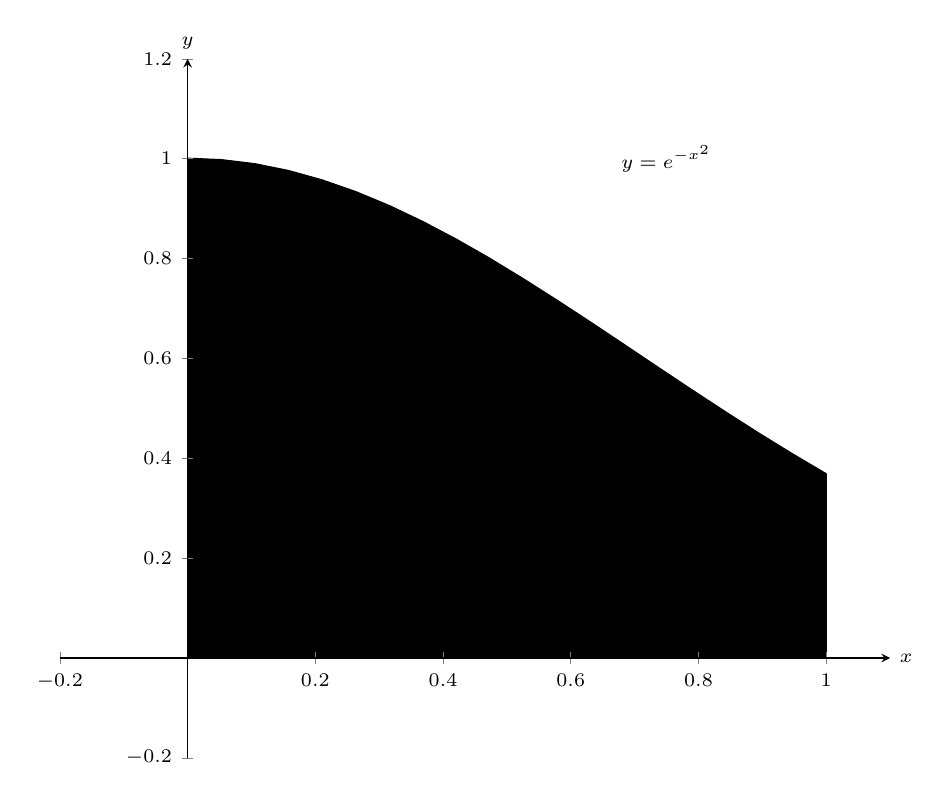
\begin{tikzpicture}
\begin{axis}[width=\textwidth,%
tick label style={font=\scriptsize},axis y line=middle,axis x line=middle,name=myplot,axis on top,%
			%x=.37\marginparwidth,
			%y=.37\marginparwidth,
%			xtick=\empty,% 
%			extra x ticks={.5,3},
%			extra x tick labels={$a$,$b$},
%			ytick=\empty,
			%minor y tick num=1,%extra y ticks={-5,-3,...,7},%
%			minor x tick num=4,
			ymin=-.2,ymax=1.2,%
			xmin=-.2,xmax=1.1%
]

\addplot [{\coloronefill},fill={\coloronefill}] coordinates {(0.0000,1.0000)  (0.0526,0.9972) (0.1053,0.9890)
(0.1579,0.9754)  (0.2105,0.9566) (0.2632,0.9331)
(0.3158,0.9051)  (0.3684,0.8731) (0.4211,0.8375)
(0.4737,0.7990)  (0.5263,0.7580) (0.5789,0.7152)
(0.6316,0.6711)  (0.6842,0.6262) (0.7368,0.5810)
(0.7895,0.5362)  (0.8421,0.4921) (0.8947,0.4491)
(0.9474,0.4076)  (1.0000,0.3679) }
|-(axis cs:0,0)--cycle;

\addplot [{\colorone},thick] coordinates {(0.0000,1.0000)  (0.0526,0.9972) (0.1053,0.9890)
(0.1579,0.9754)  (0.2105,0.9566) (0.2632,0.9331)
(0.3158,0.9051)  (0.3684,0.8731) (0.4211,0.8375)
(0.4737,0.7990)  (0.5263,0.7580) (0.5789,0.7152)
(0.6316,0.6711)  (0.6842,0.6262) (0.7368,0.5810)
(0.7895,0.5362)  (0.8421,0.4921) (0.8947,0.4491)
(0.9474,0.4076)  (1.0000,0.3679) };

\draw (axis cs:.75,1) node {\scriptsize $y=e^{-x^2}$};
\end{axis}

\node [right] at (myplot.right of origin) {\scriptsize $x$};
\node [above] at (myplot.above origin) {\scriptsize $y$};
\end{tikzpicture}
  \caption{}
  %\label{fig:numerical1}
\end{subfigure}%
\begin{subfigure}{.33\textwidth}
  \centering
  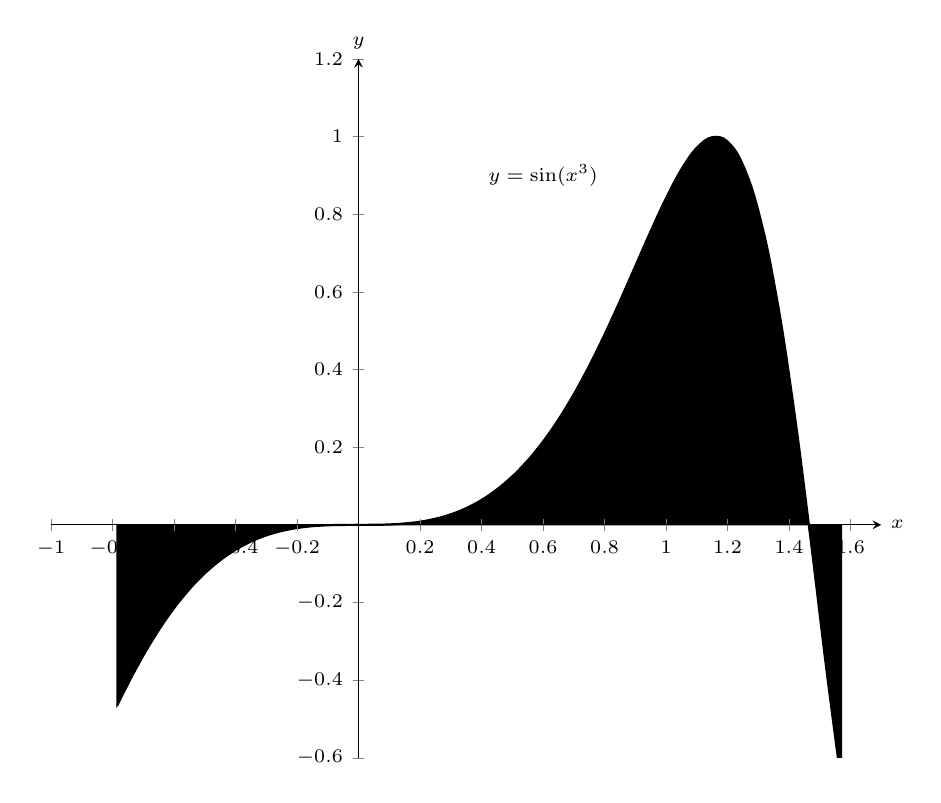
\begin{tikzpicture}
  \begin{axis}[width=\textwidth,%
  tick label style={font=\scriptsize},axis y line=middle,axis x line=middle,name=myplot,axis on top,%
  			%x=.37\marginparwidth,
  			%y=.37\marginparwidth,
  %			xtick=\empty,% 
  %			extra x ticks={.5,3},
  %			extra x tick labels={$a$,$b$},
  %			ytick=\empty,
  			%minor y tick num=1,%extra y ticks={-5,-3,...,7},%
  %			minor x tick num=4,
  			ymin=-.6,ymax=1.2,%
  			xmin=-1,xmax=1.7%
  ]
  
  \addplot [{\coloronefill},fill={\coloronefill}] coordinates {(-0.7854,-0.4657)  (-0.7373,-0.3902) (-0.6892,-0.3216)
  (-0.6411,-0.2605)  (-0.5931,-0.2071) (-0.5450,-0.1611)
  (-0.4969,-0.1224)  (-0.4488,-0.0903) (-0.4007,-0.0643)
  (-0.3526,-0.0438)  (-0.3045,-0.0282) (-0.2565,-0.0169)
  (-0.2084,-0.0090)  (-0.1603,-0.0041) (-0.1122,-0.0014)
  (-0.0641,-0.0003)  (-0.0160,-0.0000) (0.0321,0.0000)
  (0.0801,0.0005)  (0.1282,0.0021) (0.1763,0.0055)
  (0.2244,0.0113)  (0.2725,0.0202) (0.3206,0.0329)
  (0.3687,0.0501)  (0.4167,0.0723) (0.4648,0.1003)
  (0.5129,0.1345)  (0.5610,0.1756) (0.6091,0.2240)
  (0.6572,0.2800)  (0.7053,0.3436) (0.7533,0.4146)
  (0.8014,0.4923)  (0.8495,0.5754) (0.8976,0.6618)
  (0.9457,0.7485)  (0.9938,0.8313) (1.0419,0.9048)
  (1.0899,0.9622)  (1.1380,0.9953) (1.1861,0.9952)
  (1.2342,0.9526)  (1.2823,0.8589) (1.3304,0.7082)
  (1.3785,0.4989)  (1.4265,0.2363) (1.4746,-0.0650)
  (1.5227,-0.3793)  (1.5708,-0.6700) }
  |-(axis cs:-0.7854,0 )--cycle;
  
  \addplot [{\colorone},thick,smooth] coordinates {(-0.7854,-0.4657)  (-0.7373,-0.3902) (-0.6892,-0.3216)
  (-0.6411,-0.2605)  (-0.5931,-0.2071) (-0.5450,-0.1611)
  (-0.4969,-0.1224)  (-0.4488,-0.0903) (-0.4007,-0.0643)
  (-0.3526,-0.0438)  (-0.3045,-0.0282) (-0.2565,-0.0169)
  (-0.2084,-0.0090)  (-0.1603,-0.0041) (-0.1122,-0.0014)
  (-0.0641,-0.0003)  (-0.0160,-0.0000) (0.0321,0.0000)
  (0.0801,0.0005)  (0.1282,0.0021) (0.1763,0.0055)
  (0.2244,0.0113)  (0.2725,0.0202) (0.3206,0.0329)
  (0.3687,0.0501)  (0.4167,0.0723) (0.4648,0.1003)
  (0.5129,0.1345)  (0.5610,0.1756) (0.6091,0.2240)
  (0.6572,0.2800)  (0.7053,0.3436) (0.7533,0.4146)
  (0.8014,0.4923)  (0.8495,0.5754) (0.8976,0.6618)
  (0.9457,0.7485)  (0.9938,0.8313) (1.0419,0.9048)
  (1.0899,0.9622)  (1.1380,0.9953) (1.1861,0.9952)
  (1.2342,0.9526)  (1.2823,0.8589) (1.3304,0.7082)
  (1.3785,0.4989)  (1.4265,0.2363) (1.4746,-0.0650)
  (1.5227,-0.3793)  (1.5708,-0.6700) };
  
  \draw (axis cs:.6,.9) node {\scriptsize $y=\sin(x^3)$};
  \end{axis}
  
  \node [right] at (myplot.right of origin) {\scriptsize $x$};
  \node [above] at (myplot.above origin) {\scriptsize $y$};
  \end{tikzpicture}  
  \caption{}
  %\label{fig:sub2}
\end{subfigure}
\begin{subfigure}{.33\textwidth}
  \centering
  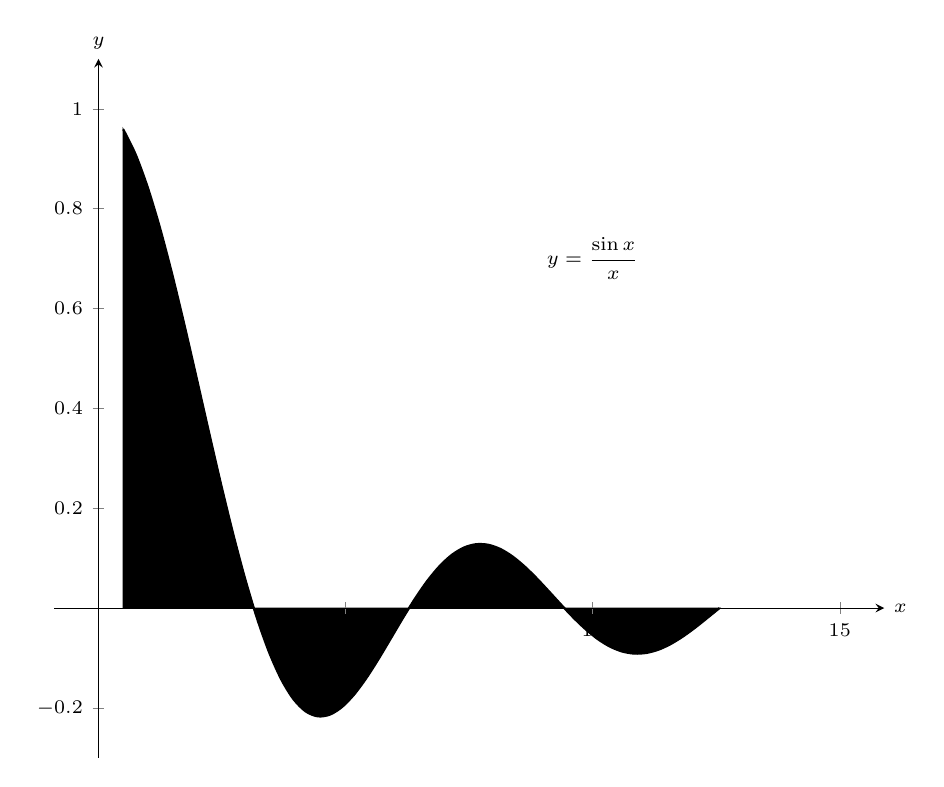
\begin{tikzpicture}
  \begin{axis}[width=\textwidth,%
  tick label style={font=\scriptsize},axis y line=middle,axis x line=middle,name=myplot,axis on top,%
  			%x=.37\marginparwidth,
  			%y=.37\marginparwidth,
  			xtick={5,10,15},% 
  %			extra x ticks={.5,3},
  %			extra x tick labels={$a$,$b$},
  %			ytick=\empty,
  			%minor y tick num=1,%extra y ticks={-5,-3,...,7},%
  %			minor x tick num=4,
  			ymin=-.3,ymax=1.1,%
  			xmin=-.9,xmax=15.9%
  ]
  
  \addplot [{\coloronefill},fill={\coloronefill}] coordinates {(0.5000,0.9589)  (0.7463,0.9097) (0.9925,0.8437)
  (1.2388,0.7632)  (1.4850,0.6709) (1.7313,0.5702)
  (1.9775,0.4644)  (2.2238,0.3572) (2.4700,0.2519)
  (2.7163,0.1519)  (2.9625,0.0601) (3.2088,-0.0209)
  (3.4550,-0.0892)  (3.7013,-0.1434) (3.9475,-0.1828)
  (4.1938,-0.2071)  (4.4400,-0.2169) (4.6863,-0.2133)
  (4.9325,-0.1978)  (5.1788,-0.1725) (5.4250,-0.1395)
  (5.6713,-0.1013)  (5.9176,-0.0604) (6.1638,-0.0193)
  (6.4101,0.0197)  (6.6563,0.0548) (6.9026,0.0841)
  (7.1488,0.1065)  (7.3951,0.1212) (7.6413,0.1279)
  (7.8876,0.1267)  (8.1338,0.1182) (8.3801,0.1032)
  (8.6263,0.0830)  (8.8726,0.0591) (9.1188,0.0330)
  (9.3651,0.0064)  (9.6113,-0.0193) (9.8576,-0.0425)
  (10.1038,-0.0622)  (10.3501,-0.0772) (10.5964,-0.0870)
  (10.8426,-0.0912)  (11.0889,-0.0898) (11.3351,-0.0832)
  (11.5814,-0.0719)  (11.8276,-0.0569) (12.0739,-0.0392)
  (12.3201,-0.0198)  (12.5664,-0.0000)}
  |-(axis cs:0.5,0)--cycle;
  
  \addplot [{\colorone},thick,smooth] coordinates {(0.5000,0.9589)  (0.7463,0.9097) (0.9925,0.8437)
  (1.2388,0.7632)  (1.4850,0.6709) (1.7313,0.5702)
  (1.9775,0.4644)  (2.2238,0.3572) (2.4700,0.2519)
  (2.7163,0.1519)  (2.9625,0.0601) (3.2088,-0.0209)
  (3.4550,-0.0892)  (3.7013,-0.1434) (3.9475,-0.1828)
  (4.1938,-0.2071)  (4.4400,-0.2169) (4.6863,-0.2133)
  (4.9325,-0.1978)  (5.1788,-0.1725) (5.4250,-0.1395)
  (5.6713,-0.1013)  (5.9176,-0.0604) (6.1638,-0.0193)
  (6.4101,0.0197)  (6.6563,0.0548) (6.9026,0.0841)
  (7.1488,0.1065)  (7.3951,0.1212) (7.6413,0.1279)
  (7.8876,0.1267)  (8.1338,0.1182) (8.3801,0.1032)
  (8.6263,0.0830)  (8.8726,0.0591) (9.1188,0.0330)
  (9.3651,0.0064)  (9.6113,-0.0193) (9.8576,-0.0425)
  (10.1038,-0.0622)  (10.3501,-0.0772) (10.5964,-0.0870)
  (10.8426,-0.0912)  (11.0889,-0.0898) (11.3351,-0.0832)
  (11.5814,-0.0719)  (11.8276,-0.0569) (12.0739,-0.0392)
  (12.3201,-0.0198)  (12.5664,-0.0000)};
  
  \draw (axis cs:10,.7) node {\scriptsize $\displaystyle y=\frac{\sin x}{x}$};
  \end{axis}
  
  \node [right] at (myplot.right of origin) {\scriptsize $x$};
  \node [above] at (myplot.above origin) {\scriptsize $y$};
  \end{tikzpicture}    
  \caption{}
  %\label{fig:sub2}
\end{subfigure}
\caption{Graphing the areas defined by the definite integrals of Example \ref{exa:ex_subst13}. \label{fig:subst13}}
\label{fig:numerical1}
\end{figure}


\subsection*{The Left Hand, Right Hand, and Midpoint Rule Methods}

In Section \ref{sec:AreaProb} we addressed the problem of evaluating definite integrals by approximating the area under the curve using rectangles. We revisit those ideas here before introducing other methods of approximating definite integrals. \index{numerical integration!Left/Right Hand Rule}\index{Right Hand Rule}\index{Left Hand Rule}\index{integration!numerical!Left/Right Hand Rule}

We start with a review of notation. Let $f$ be a continuous function on the interval $[a,b]$. We wish to approximate $\ds \int_a^b f(x)\ dx$. We partition $[a,b]$ into $n$ equally spaced subintervals, each of length $\ds \dx = \frac{b-a}{n}$. The endpoints of these subintervals are labelled as $$x_0=a,\ x_1 = a+\dx,\ x_2 = a+ 2\dx,\ \ldots,\ x_i = a+(i)\dx,\ \ldots,\ x_{n} = b.$$

To use the Left Hand Rule we use the summation $\ds \sum_{i=1}^n f(x_{i-1})\dx$,  to use the Right Hand Rule we use $\ds \sum_{i=1}^n f(x_{i})\dx$, and for the Midpoint rule we used $ \sum_{i = 1}^{n} f(\overline{x}_i) \triangle x $, where  $\overline{x}_{i} = (x_{i-1} + x_i)/2$. We review the use of the Left and Right Hand rules in the context of examples.\\


\begin{example}{Approximating definite integrals with rectangles}{ex_num1}
{
Approximate $\ds \int_0^1e^{-x^2}\ dx$ using the Left and Right Hand Rules with $ 5 $ equally spaced subintervals.
}
\end{example}

\begin{solution}
{We begin by partitioning the interval $[0,1]$ into 5 equally spaced intervals. We have $\dx = \frac{1-0}5 = 1/5=0.2$, so $$x_1 = 0,\ x_2 = 0.2,\ x_3 = 0.4,\ x_4 = 0.6,\ x_5 = 0.8,\ \text{and}\ x_6 = 1.$$

Using the Left Hand Rule, we have:

\begin{align*}
\sum_{i=1}^n f(x_{i-1})\dx &= \big(f(x_0)+f(x_1) + f(x_2) + f(x_3) + f(x_4)\big)\dx \\
												&= \big(f(0) + f(0.2) + f(0.4) + f(0.6) + f(0.8)\big)\dx \\
												&\approx \big(1+0.961 + 0.852 + 0.698 + 0.527)(0.2)\\
												&\approx 0.808.
\end{align*}

Using the Right Hand Rule, we have:

\begin{align*}
\sum_{i=1}^n f(x_{i})\dx &= \big(f(x_1) + f(x_2) + f(x_3) + f(x_4)+f(x_5)\big)\dx \\
												&= \big(f(0.2) + f(0.4) + f(0.6) + f(0.8)+f(1)\big)\dx \\
												&\approx \big(0.961 +0.852 + 0.698 + 0.527 + 0.368)(0.2)\\
												&\approx 0.681.
\end{align*}




\begin{figure}
\centering
\begin{subfigure}{.5\textwidth}
  \centering
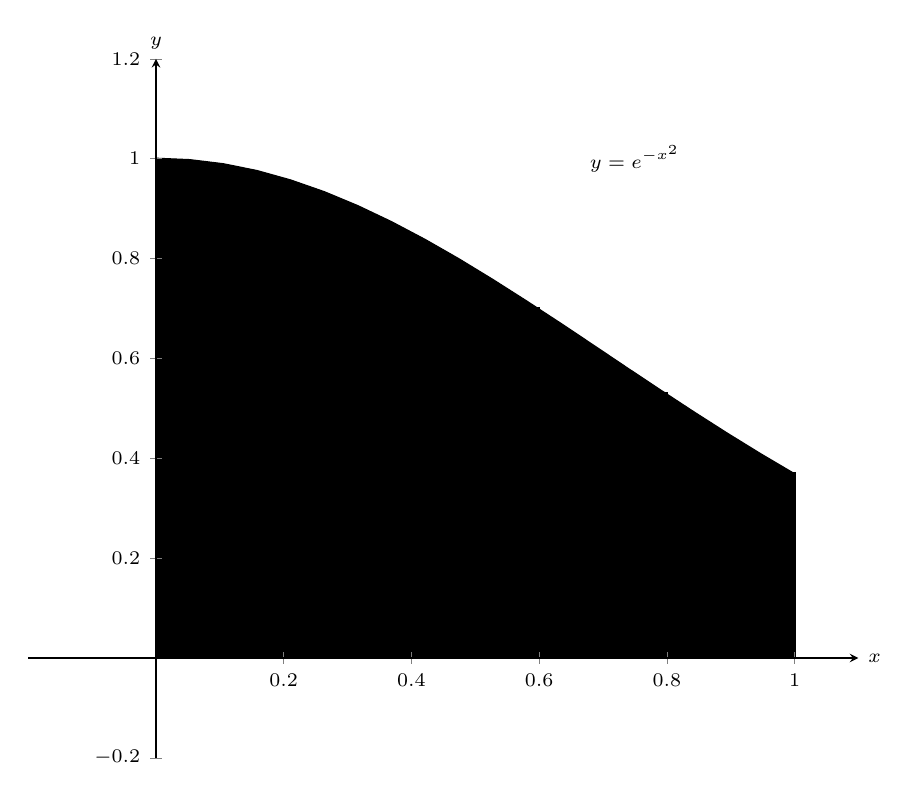
\begin{tikzpicture}
\begin{axis}[width=\textwidth,%
tick label style={font=\scriptsize},axis y line=middle,axis x line=middle,name=myplot,axis on top,%
			%x=.37\marginparwidth,
			%y=.37\marginparwidth,
			xtick={.2,.4,.6,.8,1},% 
%			extra x ticks={.5,3},
%			extra x tick labels={$a$,$b$},
%			ytick=\empty,
			%minor y tick num=1,%extra y ticks={-5,-3,...,7},%
%			minor x tick num=4,
			ymin=-.2,ymax=1.2,%
			xmin=-.2,xmax=1.1%
]

\addplot [{\coloronefill},fill={\coloronefill}] coordinates {(0.0000,1.0000)  (0.0526,0.9972) (0.1053,0.9890)
(0.1579,0.9754)  (0.2105,0.9566) (0.2632,0.9331)
(0.3158,0.9051)  (0.3684,0.8731) (0.4211,0.8375)
(0.4737,0.7990)  (0.5263,0.7580) (0.5789,0.7152)
(0.6316,0.6711)  (0.6842,0.6262) (0.7368,0.5810)
(0.7895,0.5362)  (0.8421,0.4921) (0.8947,0.4491)
(0.9474,0.4076)  (1.0000,0.3679) }
|-(axis cs:0,0)--cycle;

\addplot [{\colorone},thick] coordinates {(0.0000,1.0000)  (0.0526,0.9972) (0.1053,0.9890)
(0.1579,0.9754)  (0.2105,0.9566) (0.2632,0.9331)
(0.3158,0.9051)  (0.3684,0.8731) (0.4211,0.8375)
(0.4737,0.7990)  (0.5263,0.7580) (0.5789,0.7152)
(0.6316,0.6711)  (0.6842,0.6262) (0.7368,0.5810)
(0.7895,0.5362)  (0.8421,0.4921) (0.8947,0.4491)
(0.9474,0.4076)  (1.0000,0.3679) };

\foreach \x / \y in {0.2 / 0.96, 0.4 / .85, 0.6 / .7, .8 / .53, 1/ .37}
  	{\addplot [thick,draw={\colortwo}] coordinates {(\x-.2,0) (\x-.2,\y) (\x,\y) (\x,0) (\x-.2,0)};
  	}

\draw (axis cs:.75,1) node {\scriptsize $y=e^{-x^2}$};
\end{axis}

\node [right] at (myplot.right of origin) {\scriptsize $x$};
\node [above] at (myplot.above origin) {\scriptsize $y$};
\end{tikzpicture}

  \caption{}
  %\label{fig:numerical1}
\end{subfigure}%
\begin{subfigure}{.5\textwidth}
  \centering
  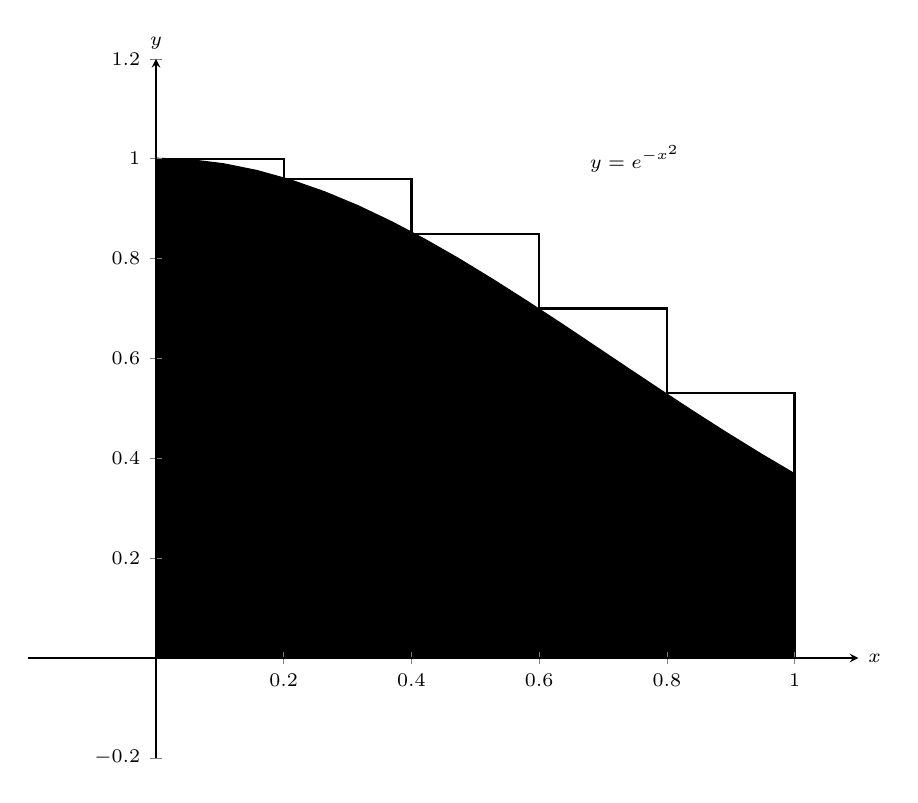
\begin{tikzpicture}
  \begin{axis}[width=\textwidth,%
  tick label style={font=\scriptsize},axis y line=middle,axis x line=middle,name=myplot,axis on top,%
  			%x=.37\marginparwidth,
  			%y=.37\marginparwidth,
  			xtick={.2,.4,.6,.8,1},% 
  %			extra x ticks={.5,3},
  %			extra x tick labels={$a$,$b$},
  %			ytick=\empty,
  			%minor y tick num=1,%extra y ticks={-5,-3,...,7},%
  %			minor x tick num=4,
  			ymin=-.2,ymax=1.2,%
  			xmin=-.2,xmax=1.1%
  ]
  
  \addplot [{\coloronefill},fill={\coloronefill}] coordinates {(0.0000,1.0000)  (0.0526,0.9972) (0.1053,0.9890)
  (0.1579,0.9754)  (0.2105,0.9566) (0.2632,0.9331)
  (0.3158,0.9051)  (0.3684,0.8731) (0.4211,0.8375)
  (0.4737,0.7990)  (0.5263,0.7580) (0.5789,0.7152)
  (0.6316,0.6711)  (0.6842,0.6262) (0.7368,0.5810)
  (0.7895,0.5362)  (0.8421,0.4921) (0.8947,0.4491)
  (0.9474,0.4076)  (1.0000,0.3679) }
  |-(axis cs:0,0)--cycle;
  
  \addplot [{\colorone},thick] coordinates {(0.0000,1.0000)  (0.0526,0.9972) (0.1053,0.9890)
  (0.1579,0.9754)  (0.2105,0.9566) (0.2632,0.9331)
  (0.3158,0.9051)  (0.3684,0.8731) (0.4211,0.8375)
  (0.4737,0.7990)  (0.5263,0.7580) (0.5789,0.7152)
  (0.6316,0.6711)  (0.6842,0.6262) (0.7368,0.5810)
  (0.7895,0.5362)  (0.8421,0.4921) (0.8947,0.4491)
  (0.9474,0.4076)  (1.0000,0.3679) };
  
  \foreach \x / \y in {0 / 1, 0.2 / 0.96, 0.4 / .85, 0.6 / .7, .8 / .53}
    	{\addplot [thick,draw={\colortwo}] coordinates {(\x+.2,0) (\x+.2,\y) (\x,\y) (\x,0) (\x+.2,0)};
    	}
  
  \draw (axis cs:.75,1) node {\scriptsize $y=e^{-x^2}$};
  \end{axis}
  
  \node [right] at (myplot.right of origin) {\scriptsize $x$};
  \node [above] at (myplot.above origin) {\scriptsize $y$};
  \end{tikzpicture}
  
  \caption{}
  %\label{fig:sub2}
\end{subfigure}
\caption{Approximating $\int_0^1e^{-x^2}\ dx$ in Example \ref{exa:ex_num1}. \label{fig:num1}}
\end{figure}

%\mtable{.6}{Approximating $\int_0^1e^{-x^2}\ dx$ in Example \ref{ex_num1}.}{fig:num1}{\myincludegraphics{figures/fignum1b}\vskip 25pt \myincludegraphics{figures/fignum1a}}

Figure \ref{fig:num1} shows the rectangles used in each method to approximate the definite integral. These graphs show that in this particular case, the Left Hand Rule is an over approximation and the Right Hand Rule is an under approximation. To get a better approximation, we could use more rectangles. We could also average the Left and Right Hand Rule results together, giving $$ \frac{0.808 + 0.681}{2} = 0.7445.$$ The actual answer, accurate to $ 4 $ places after the decimal, is $ 0.7468 $, showing our average is a good approximation.
}\\
\end{solution}






\begin{example}{Approximating definite integrals with rectangles}{ex_num2}{
Approximate $\ds\int_{-\frac{\pi}4}^{\frac{\pi}2} \sin (x^3)\ dx$ using the Left and Right Hand Rules with $ 10 $ equally spaced subintervals.}
\end{example}

\begin{solution}
{We begin by finding \dx:
$$\frac{b-a}{n} = \frac{\pi/2 - (-\pi/4)}{10} = \frac{3\pi}{40}\approx 0.236.$$
It is useful to write out the endpoints of the subintervals in a table; in Figure \ref{fig:num2a}, we give the exact values of the endpoints, their decimal approximations, and decimal approximations of $\sin(x^3)$ evaluated at these points. 

\mtable{.8}{Table of values used to approximate $\int_{-\frac{\pi}4}^{\frac{\pi}2}\sin(x^3)\ dx$ in Example \ref{exa:ex_num2}.}{fig:num2a}{%
	\begin{tabular}{cccc} 
	$x_i$ & Exact & Approx. & $\sin(x_i^3)$ \\ \hline
	$x_0$ & $-\pi/4$ & $-0.785$ & $-0.466$ \\
 $x_1$ & $-7 \pi/40$ & $-0.550$ & $-0.165$
   \\
 $x_2$ & $-{\pi }/{10}$ & $-0.314$ & $-0.031$ \\
 $x_3$ & $-{\pi }/{40}$ & $-0.0785$ & $0$
   \\
 $x_4$ & ${\pi }/{20}$ & 0.157 & 0.004 \\
 $x_5$ & ${\pi }/{8}$ & 0.393 & 0.061 \\
 $x_6$ & ${\pi }/{5}$ & 0.628 & 0.246 \\
 $x_7$ & ${11 \pi }/{40}$ & 0.864 & 0.601 \\
 $x_8$ & ${7 \pi }/{20}$ & 1.10 & 0.971 \\
 $x_{9}$ & ${17 \pi }/{40}$ & 1.34 & 0.690 \\
 $x_{10}$ & ${\pi }/{2}$ & 1.57 & $-0.670$ \\
	\end{tabular}
}
Once this table is created, it is straightforward to approximate the definite integral using the Left and Right Hand Rules. (Note: the table itself is easy to create, especially with a standard spreadsheet program on a computer. The last two columns are all that are needed.) The Left Hand Rule sums the first 10 values of $\sin(x_i^3)$ and multiplies the sum by $\dx$; the Right Hand Rule sums the last 10 values of $\sin(x_i^3)$ and multiplies by $\dx$. Therefore we have:

Left Hand Rule: $\ds \int_{-\frac{\pi}4}^{\frac{\pi}2}\sin(x^3)\ dx \approx (1.91)(0.236) = 0.451.$

Right Hand Rule: $\ds \int_{-\frac{\pi}4}^{\frac{\pi}2}\sin(x^3)\ dx \approx (1.71)(0.236) = 0.404.$

Average of the Left and Right Hand Rules: 0.4275.


\mtable{.45}{Approximating $\int_{-\frac{\pi}4}^{\frac{\pi}2}\sin(x^3)\ dx$ in Example \ref{ex_num2}.}{fig:num2b}{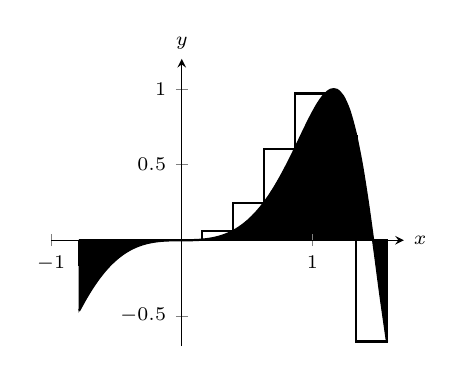
\begin{tikzpicture}
\begin{axis}[width=.5\textwidth,%
tick label style={font=\scriptsize},axis y line=middle,axis x line=middle,name=myplot,axis on top,%
			%x=.37\marginparwidth,
			%y=.37\marginparwidth,
%			xtick=\empty,% 
%			extra x ticks={.5,3},
%			extra x tick labels={$a$,$b$},
%			ytick=\empty,
			%minor y tick num=1,%extra y ticks={-5,-3,...,7},%
%			minor x tick num=4,
			ymin=-.7,ymax=1.2,%
			xmin=-1,xmax=1.7%
]

\addplot [{\coloronefill},fill={\coloronefill}] coordinates {(-0.7854,-0.4657)  (-0.7373,-0.3902) (-0.6892,-0.3216)
(-0.6411,-0.2605)  (-0.5931,-0.2071) (-0.5450,-0.1611)
(-0.4969,-0.1224)  (-0.4488,-0.0903) (-0.4007,-0.0643)
(-0.3526,-0.0438)  (-0.3045,-0.0282) (-0.2565,-0.0169)
(-0.2084,-0.0090)  (-0.1603,-0.0041) (-0.1122,-0.0014)
(-0.0641,-0.0003)  (-0.0160,-0.0000) (0.0321,0.0000)
(0.0801,0.0005)  (0.1282,0.0021) (0.1763,0.0055)
(0.2244,0.0113)  (0.2725,0.0202) (0.3206,0.0329)
(0.3687,0.0501)  (0.4167,0.0723) (0.4648,0.1003)
(0.5129,0.1345)  (0.5610,0.1756) (0.6091,0.2240)
(0.6572,0.2800)  (0.7053,0.3436) (0.7533,0.4146)
(0.8014,0.4923)  (0.8495,0.5754) (0.8976,0.6618)
(0.9457,0.7485)  (0.9938,0.8313) (1.0419,0.9048)
(1.0899,0.9622)  (1.1380,0.9953) (1.1861,0.9952)
(1.2342,0.9526)  (1.2823,0.8589) (1.3304,0.7082)
(1.3785,0.4989)  (1.4265,0.2363) (1.4746,-0.0650)
(1.5227,-0.3793)  (1.5708,-0.6700) }
|-(axis cs:-0.7854,0 )--cycle;

\addplot [{\colorone},thick,smooth] coordinates {(-0.7854,-0.4657)  (-0.7373,-0.3902) (-0.6892,-0.3216)
(-0.6411,-0.2605)  (-0.5931,-0.2071) (-0.5450,-0.1611)
(-0.4969,-0.1224)  (-0.4488,-0.0903) (-0.4007,-0.0643)
(-0.3526,-0.0438)  (-0.3045,-0.0282) (-0.2565,-0.0169)
(-0.2084,-0.0090)  (-0.1603,-0.0041) (-0.1122,-0.0014)
(-0.0641,-0.0003)  (-0.0160,-0.0000) (0.0321,0.0000)
(0.0801,0.0005)  (0.1282,0.0021) (0.1763,0.0055)
(0.2244,0.0113)  (0.2725,0.0202) (0.3206,0.0329)
(0.3687,0.0501)  (0.4167,0.0723) (0.4648,0.1003)
(0.5129,0.1345)  (0.5610,0.1756) (0.6091,0.2240)
(0.6572,0.2800)  (0.7053,0.3436) (0.7533,0.4146)
(0.8014,0.4923)  (0.8495,0.5754) (0.8976,0.6618)
(0.9457,0.7485)  (0.9938,0.8313) (1.0419,0.9048)
(1.0899,0.9622)  (1.1380,0.9953) (1.1861,0.9952)
(1.2342,0.9526)  (1.2823,0.8589) (1.3304,0.7082)
(1.3785,0.4989)  (1.4265,0.2363) (1.4746,-0.0650)
(1.5227,-0.3793)  (1.5708,-0.6700) };

\foreach \x / \y in %
		{-0.550/-0.165, -0.314/ -0.0310,%
		 -0.0785/-0.000484, 0.157/ 0.00388, 0.393/ 0.0605,
		 0.628/ 0.246, 0.864/ 0.601, 1.10/ 0.971, 1.34/ 0.690, 1.57/ -0.670}
  	{\addplot [thick,draw={\colortwo}] coordinates {(\x-.2356,0) (\x-.2356,\y) (\x,\y) (\x,0) (\x-.2356,0)};
  	}

%\draw (axis cs:.6,1.1) node {\scriptsize $y=\sin(x^3)$};
\end{axis}

\node [right] at (myplot.right of origin) {\scriptsize $x$};
\node [above] at (myplot.above origin) {\scriptsize $y$};
\end{tikzpicture}\hspace*{4mm} 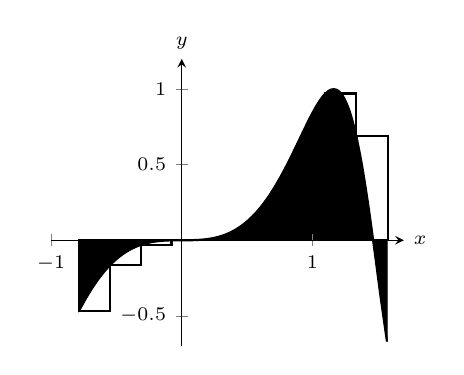
\begin{tikzpicture}
\begin{axis}[width=.5\textwidth,%
tick label style={font=\scriptsize},axis y line=middle,axis x line=middle,name=myplot,axis on top,%
			%x=.37\marginparwidth,
			%y=.37\marginparwidth,
%			xtick=\empty,% 
%			extra x ticks={.5,3},
%			extra x tick labels={$a$,$b$},
%			ytick=\empty,
			%minor y tick num=1,%extra y ticks={-5,-3,...,7},%
%			minor x tick num=4,
			ymin=-.7,ymax=1.2,%
			xmin=-1,xmax=1.7%
]

\addplot [{\coloronefill},fill={\coloronefill}] coordinates {(-0.7854,-0.4657)  (-0.7373,-0.3902) (-0.6892,-0.3216)
(-0.6411,-0.2605)  (-0.5931,-0.2071) (-0.5450,-0.1611)
(-0.4969,-0.1224)  (-0.4488,-0.0903) (-0.4007,-0.0643)
(-0.3526,-0.0438)  (-0.3045,-0.0282) (-0.2565,-0.0169)
(-0.2084,-0.0090)  (-0.1603,-0.0041) (-0.1122,-0.0014)
(-0.0641,-0.0003)  (-0.0160,-0.0000) (0.0321,0.0000)
(0.0801,0.0005)  (0.1282,0.0021) (0.1763,0.0055)
(0.2244,0.0113)  (0.2725,0.0202) (0.3206,0.0329)
(0.3687,0.0501)  (0.4167,0.0723) (0.4648,0.1003)
(0.5129,0.1345)  (0.5610,0.1756) (0.6091,0.2240)
(0.6572,0.2800)  (0.7053,0.3436) (0.7533,0.4146)
(0.8014,0.4923)  (0.8495,0.5754) (0.8976,0.6618)
(0.9457,0.7485)  (0.9938,0.8313) (1.0419,0.9048)
(1.0899,0.9622)  (1.1380,0.9953) (1.1861,0.9952)
(1.2342,0.9526)  (1.2823,0.8589) (1.3304,0.7082)
(1.3785,0.4989)  (1.4265,0.2363) (1.4746,-0.0650)
(1.5227,-0.3793)  (1.5708,-0.6700) }
|-(axis cs:-0.7854,0 )--cycle;

\addplot [{\colorone},thick,smooth] coordinates {(-0.7854,-0.4657)  (-0.7373,-0.3902) (-0.6892,-0.3216)
(-0.6411,-0.2605)  (-0.5931,-0.2071) (-0.5450,-0.1611)
(-0.4969,-0.1224)  (-0.4488,-0.0903) (-0.4007,-0.0643)
(-0.3526,-0.0438)  (-0.3045,-0.0282) (-0.2565,-0.0169)
(-0.2084,-0.0090)  (-0.1603,-0.0041) (-0.1122,-0.0014)
(-0.0641,-0.0003)  (-0.0160,-0.0000) (0.0321,0.0000)
(0.0801,0.0005)  (0.1282,0.0021) (0.1763,0.0055)
(0.2244,0.0113)  (0.2725,0.0202) (0.3206,0.0329)
(0.3687,0.0501)  (0.4167,0.0723) (0.4648,0.1003)
(0.5129,0.1345)  (0.5610,0.1756) (0.6091,0.2240)
(0.6572,0.2800)  (0.7053,0.3436) (0.7533,0.4146)
(0.8014,0.4923)  (0.8495,0.5754) (0.8976,0.6618)
(0.9457,0.7485)  (0.9938,0.8313) (1.0419,0.9048)
(1.0899,0.9622)  (1.1380,0.9953) (1.1861,0.9952)
(1.2342,0.9526)  (1.2823,0.8589) (1.3304,0.7082)
(1.3785,0.4989)  (1.4265,0.2363) (1.4746,-0.0650)
(1.5227,-0.3793)  (1.5708,-0.6700) };

\foreach \x / \y in %
		{-0.785/ -0.466, -0.550/-0.165, -0.314/ -0.0310,%
		 -0.0785/-0.000484, 0.157/ 0.00388, 0.393/ 0.0605,
		 0.628/ 0.246, 0.864/ 0.601, 1.10/ 0.971, 1.34/ 0.690}
  	{\addplot [thick,draw={\colortwo}] coordinates {(\x+.2356,0) (\x+.2356,\y) (\x,\y) (\x,0) (\x+.2356,0)};
  	}

%\draw (axis cs:.6,.9) node {\scriptsize $y=\sin(x^3)$};
\end{axis}

\node [right] at (myplot.right of origin) {\scriptsize $x$};
\node [above] at (myplot.above origin) {\scriptsize $y$};
\end{tikzpicture}
}



The actual answer, accurate to 3 places after the decimal, is 0.460. Our approximations were once again fairly good. The rectangles used in each approximation are shown in Figure \ref{fig:num2b}. It is clear from the graphs that using more rectangles (and hence, narrower rectangles) should result in a more accurate approximation.
}
\end{solution}





\subsection{The Trapezoidal Rule}

In Example \ref{ex_num1} we approximated the value of $\ds \int_0^1 e^{-x^2}\ dx$ with 5 rectangles of equal width. Figure \ref{fig:num1} shows the rectangles used in the Left and Right Hand Rules. These graphs clearly show that rectangles do not match the shape of the graph all that well, and that accurate approximations will only come by using lots of rectangles. \index{Trapezoidal Rule}\index{numerical integration!Trapezoidal Rule}\index{integration!numerical!Trapezoidal Rule}

Instead of using rectangles to approximate the area, we can instead use \textit{trapezoids.} In Figure \ref{fig:num3a}, we show the region under $f(x) = e^{-x^2}$ on $[0,1]$ approximated with 5 trapezoids of equal width; the top ``corners'' of each trapezoid lies on the graph of $f(x)$. It is clear from this figure that these trapezoids more accurately approximate the area under $f$ and hence should give a better approximation of $\int_0^1 e^{-x^2}\ dx$. (In fact, these trapezoids seem to give a \textit{great} approximation of the area!)

\mfigure{1}{Approximating $\int_0^1 e^{-x^2}\ dx$ using 5 trapezoids of equal widths.}{fig:num3a}{
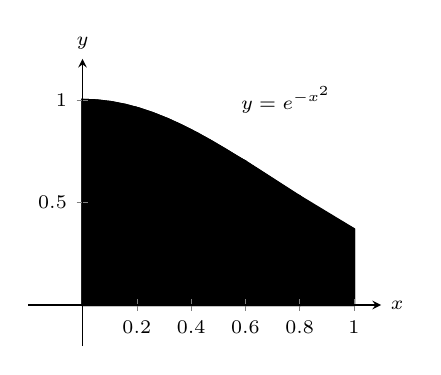
\begin{tikzpicture}
\begin{axis}[width=.5\textwidth,%
tick label style={font=\scriptsize},axis y line=middle,axis x line=middle,name=myplot,axis on top,%
			%x=.37\marginparwidth,
			%y=.37\marginparwidth,
			xtick={.2,.4,.6,.8,1},% 
%			extra x ticks={.5,3},
%			extra x tick labels={$a$,$b$},
%			ytick=\empty,
			%minor y tick num=1,%extra y ticks={-5,-3,...,7},%
%			minor x tick num=4,
			ymin=-.2,ymax=1.2,%
			xmin=-.2,xmax=1.1%
]

\addplot [{\coloronefill},fill={\coloronefill},thick] coordinates {(0.0000,1.0000)  (0.0526,0.9972) (0.1053,0.9890)
(0.1579,0.9754)  (0.2105,0.9566) (0.2632,0.9331)
(0.3158,0.9051)  (0.3684,0.8731) (0.4211,0.8375)
(0.4737,0.7990)  (0.5263,0.7580) (0.5789,0.7152)
(0.6316,0.6711)  (0.6842,0.6262) (0.7368,0.5810)
(0.7895,0.5362)  (0.8421,0.4921) (0.8947,0.4491)
(0.9474,0.4076)  (1.0000,0.3679) }
|-(axis cs:0,0)--cycle;

\addplot [{\colorone},thick] coordinates {(0.0000,1.0000)  (0.0526,0.9972) (0.1053,0.9890)
(0.1579,0.9754)  (0.2105,0.9566) (0.2632,0.9331)
(0.3158,0.9051)  (0.3684,0.8731) (0.4211,0.8375)
(0.4737,0.7990)  (0.5263,0.7580) (0.5789,0.7152)
(0.6316,0.6711)  (0.6842,0.6262) (0.7368,0.5810)
(0.7895,0.5362)  (0.8421,0.4921) (0.8947,0.4491)
(0.9474,0.4076)  (1.0000,0.3679) };

\foreach \x / \y / \z in {0/1 /0.96 , 0.2/0.96 / .85, 0.4 /.85 / .7, .6 / .7/ .53, .8 / .53 / .37}
  	{\addplot [thick,draw={\colortwo}] coordinates {(\x,0) (\x,\y) (\x+.2,\z) (\x+.2,0) (\x,0)};
  	}

\draw (axis cs:.75,1) node {\scriptsize $y=e^{-x^2}$};
\end{axis}

\node [right] at (myplot.right of origin) {\scriptsize $x$};
\node [above] at (myplot.above origin) {\scriptsize $y$};
\end{tikzpicture}
}

The formula for the area of a trapezoid is given in Figure \ref{fig:trapezoid}.


\begin{figure}
\begin{center}
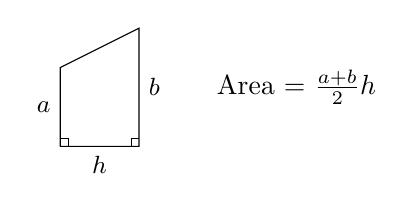
\begin{tikzpicture}
\draw (0,0) -- node [pos=.5,left] {\small $a$} (0,1) -- (1,1.5) -- node [pos=.5,right] {\small $b$} (1,0) -- node [pos=.5,below] {\small $h$} (0,0);

\draw (0,.1) -- (.1,.1) -- (.1,0);
\draw (.9,0) -- (.9,.1) -- (1,.1);

\draw (3,.75) node {Area = $\ds \frac{a+b}2h$};
\end{tikzpicture}
\caption{The area of a trapezoid. \label{fig:trapezoid}}
\end{center}
\end{figure}


 We approximate $\int_0^1 e^{-x^2}\ dx$ with these trapezoids in the following example.\\



\begin{example}{Approximating definite integrals using trapezoids}{ex_num3}
{
Use $ 5 $ trapezoids of equal width to approximate $\ds \int_0^1e^{-x^2}\ dx$.}
\end{example}

\begin{solution}
{To compute the areas of the 5 trapezoids in Figure \ref{fig:num3a}, it will again be useful to create a table of values as shown in Figure \ref{fig:num3b}.



%\mfigure{.55}{The area of a trapezoid.}{fig:trapezoid}{figures/figtrapezoid}
\mtable{.4}{A table of values of $e^{-x^2}$.}{fig:num3b}{%
\begin{tabular}{cc}
$x_i$ & $e^{-x_i^2}$ \\ \hline
0 & 1\\
0.2 & 0.961 \\
0.4 & 0.852 \\
0.6 & 0.698 \\
0.8 & 0.527 \\
1 & 0.368
\end{tabular}
}

The leftmost trapezoid has legs of length 1 and 0.961 and a height of 0.2. Thus, by our formula, the area of the leftmost trapezoid is: $$ \frac{1+0.961}{2}(0.2) = 0.1961.$$
Moving right, the next trapezoid has legs of length 0.961 and 0.852 and a height of 0.2. Thus its area is: $$\frac{0.961+0.852}2(0.2) = 0.1813.$$

The sum of the areas of all 5 trapezoids is:
%\small$$ 
\begin{align*}
\frac{1+0.961}{2}(0.2) + \frac{0.961+0.852}2(0.2)+\frac{0.852+0.698}2(0.2)&+ \\
\frac{0.698+0.527}2(0.2)+\frac{0.527+0.368}2(0.2)&= 0.7445.
\end{align*}
%$$\normalsize
We approximate $\ds \int_0^1 e^{-x^2}\ dx \approx 0.7445.$
}
\end{solution}




%
There are many things to observe in this example. Note how each term in the final summation was multiplied by both $ 1/2 $ and by $\dx = 0.2$. We can factor these coefficients out, leaving a more concise summation as:\small
$$
\frac12(0.2)\Big[(1+0.961) + (0.961+0.852) + (0.852+0.698) + ( 0.698+ 0.527) +(0.527 + 0.368)\Big].$$
\normalsize
Now notice that all numbers except for the first and the last are added twice. Therefore we can write the summation even more concisely as
$$\frac{0.2}{2}\Big[1 + 2(0.961+0.852+0.698+0.527) + 0.368\Big].$$

This is the heart of the \textbf{Trapezoidal Rule}, wherein a definite integral $\ds \int_a^b f(x) \ dx$ is approximated by using trapezoids of equal widths to approximate the corresponding area under $f$. Using $n$ equally spaced subintervals with endpoints $x_1$, $x_2$, $\ldots$, $x_{n+1}$, we again have $\ds \dx = \frac{b-a}n$. Thus:
\begin{align*}
\int_a^b f(x)\ dx & \approx \sum_{i=1}^n \frac{f(x_i)+f(x_{i+1})}2\dx \\
									& = \frac{\dx}2 \sum_{i=1}^n \big(f(x_i)+f(x_{i+1})\big)\\
									& = \frac{\dx}2\Big[f(x_1)+ 2\sum_{i=2}^n f(x_i) + f(x_{n+1})\Big].\\ 
\end{align*}


\begin{example}{Using the Trapezoidal Rule}{ex_num4}{
Revisit Example \ref{exa:ex_num2} 
and approximate $\ds\int_{-\frac{\pi}{4}}^{\frac{\pi}{2}} \sin (x^3)\ dx$ using the Trapezoidal Rule and $ 10 $ equally spaced subintervals.}
\end{example}

\begin{solution}
{We refer back to Figure \ref{fig:num2a} for the table of values of $\sin(x^3)$. Recall that $\dx = 3\pi/40 \approx 0.236$. Thus we have:\small
\begin{align*}
\int_{-\frac{\pi}4}^{\frac{\pi}2} \sin (x^3)\ dx &\approx \frac{0.236}{2}\Big[-0.466 + 2\Big(-0.165+(-0.031)+\ldots+%0.971+
0.69\Big)+(-0.67)\Big]\\
			&= 0.4275.
\end{align*}
}
\end{solution}





Notice how ``quickly'' the Trapezoidal Rule can be implemented once the table of values is created. This is true for all the methods explored in this section; the real work is creating a table of $x_i$ and $f(x_i)$ values. Once this is completed, approximating the definite integral is not difficult. Again, using technology is wise. Spreadsheets can make quick work of these computations and make using lots of subintervals easy. 

Also notice the  approximations the Trapezoidal Rule gives. It is  the average of the approximations given by the Left and Right Hand Rules! This effectively renders the Left and Right Hand Rules obsolete. They are useful when first learning about definite integrals, but if a real approximation is needed, one is generally better off using the Trapezoidal Rule instead of either the Left or Right Hand Rule.\\

How can we improve on the Trapezoidal Rule, apart from using more and more trapezoids? The answer is clear once we look back and consider what we have \textit{really} done so far. The Left Hand Rule is not \textit{really} about using rectangles to approximate area. Instead, it approximates a function $f$ with constant functions on small subintervals and then computes the definite integral of these constant functions. The Trapezoidal Rule is really approximating a function $f$ with a linear function on a small subinterval, then computes the definite integral of this linear function. In both of these cases the definite integrals are easy to compute in geometric terms.

So we have a progression: we start by approximating $f$ with a constant function and then with a linear function. What is next? A quadratic function. By approximating the curve of a function with lots of parabolas, we generally get an even better approximation of the definite integral. We call this process \textbf{Simpson's Rule}, named after Thomas Simpson (1710-1761), even though others had used this rule as much as 100 years prior.\\

\subsection{ Simpson's Rule}


Given one point, we can create a constant function that goes through that point. Given two points, we can create a linear function that goes through those points. Given three points, we can create a quadratic function that goes through those three points (given that no two have the same $x$--value).\index{Simpson's Rule}\index{numerical integration!Simpson's Rule}\index{integration!numerical!Simpson's Rule}

Consider three points $(x_1,y_1)$, $(x_2,y_2)$ and $(x_3,y_3)$ whose $x$--values are equally spaced and $x_1<x_2<x_3$. Let $f$ be the quadratic function that goes through these three points. It is not hard to show that 
\begin{equation}
\int_{x_1}^{x_3} f(x)\ dx = \frac{x_3-x_1}{6}\big(y_1+4y_2+y_3\big).\label{eq:simpsons}
\end{equation}

Consider Figure \ref{fig:numsimpsons}. A function $f$ goes through the 3 points shown and the parabola $g$ that also goes through those points is graphed with a dashed line. Using our equation from above, we know exactly that $$\int_1^3 g(x) \ dx = \frac{3-1}{6}\big(3+4(1)+2\big)= 3.$$ Since $g$ is a good approximation for $f$ on $[1,3]$, we can state that $$\int_1^3 f(x)\ dx \approx 3.$$

\mfigure{.5}{A graph of a function $f$ and a parabola that approximates it well on $[1,3]$.}{fig:numsimpsons}{
\begin{tikzpicture}
\begin{axis}[width=\marginparwidth+25pt,%
tick label style={font=\scriptsize},axis y line=middle,axis x line=middle,name=myplot,axis on top,%
			%x=.37\marginparwidth,
			%y=.37\marginparwidth,
			xtick={1,2,3},% 
%			extra x ticks={1,2,3},
%			extra x tick labels={$x_1$,$x_2$,$x_3$},
			ytick={1,2,3},
			%minor y tick num=1,%extra y ticks={-5,-3,...,7},%
%			minor x tick num=4,
			ymin=-.2,ymax=4,%
			xmin=.5,xmax=3.5%
]

\addplot [{\colorone},domain=.9:3.1,thick] {11-12*x+4.5*x^2-.5*x^3};
\addplot [{\colortwo},dashed,domain=.9:3.1,thick] {8-6.5*x+1.5*x^2};

\filldraw (axis cs:1,3) circle (1pt);
\filldraw (axis cs:2,1) circle (1pt);
\filldraw (axis cs:3,2) circle (1pt);

\end{axis}

\node [right] at (myplot.right of origin) {\scriptsize $x$};
\node [above] at (myplot.above origin) {\scriptsize $y$};
\end{tikzpicture}
}

Notice how the interval $[1,3]$ was split into two subintervals as we needed 3 points. Because of this, whenever we use Simpson's Rule, we need to break the interval into an even number of subintervals. 

In general, to approximate $\ds \int_a^b f(x)\ dx$ using Simpson's Rule, subdivide $[a,b]$ into $n$ subintervals, where $n$ is even and each subinterval has width $\dx = (b-a)/n$. We approximate $f$ with $n/2$ parabolic curves, using Equation \eqref{eq:simpsons} to compute the area under these parabolas. Adding up these areas gives the formula:
$$\int_a^b f(x) \ dx \approx \frac{\dx}3\Big[f(x_0)+4f(x_1)+2f(x_2)+4f(x_3)+\ldots+2f(x_{n-2})+4f(x_{n-1})+f(x_{n})\Big].$$
Note how the coefficients of the terms in the summation have the pattern $ 1, 4, 2, 4, 2, 4, \ldots , 2, 4, 1 $.

Let's demonstrate Simpson's Rule with a concrete example.\\


\begin{example}{Using Simpson's Rule}{ex_num5}{
Approximate $\ds\int_0^1 e^{-x^2}\ dx$ using Simpson's Rule and 4 equally spaced subintervals.}
\end{example}

\begin{solution}
{We begin by making a table of values as we have in the past, as shown in Figure \ref{fig:num5a}(a).
\mtable{.7}{A table of values to approximate $\int_0^1e^{-x^2}\ dx$, along with a graph of the function.}{fig:num5a}{%



\begin{tabular}{c}
\begin{tabular}{cc}
$x_i$ & $e^{-x_i^2}$ \\ \hline
0 & 1 \\
0.25 & 0.939 \\
0.5 & 0.779 \\
0.75 & 0.570 \\
1 & 0.368\\[10pt]
\end{tabular}\\[10pt]
(a)\\[10pt]
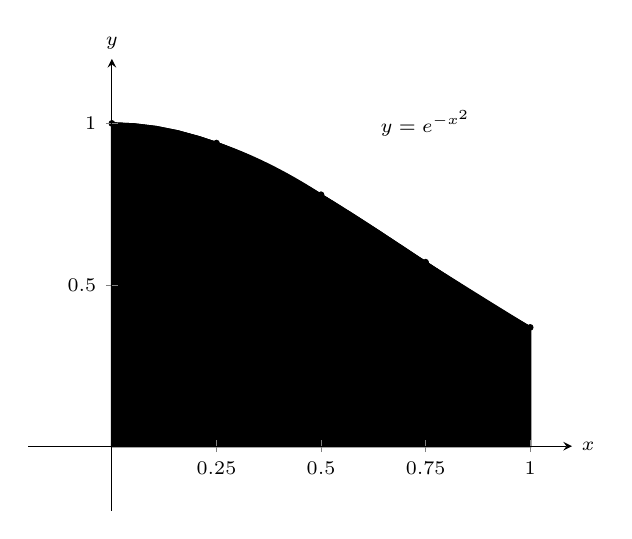
\begin{tikzpicture}
\begin{axis}[width=.7\textwidth,%
tick label style={font=\scriptsize},axis y line=middle,axis x line=middle,name=myplot,axis on top,%
			%x=.37\marginparwidth,
			%y=.37\marginparwidth,
			xtick={.25,.5,.75,1},% 
%			extra x ticks={.5,3},
%			extra x tick labels={$a$,$b$},
%			ytick=\empty,
			%minor y tick num=1,%extra y ticks={-5,-3,...,7},%
%			minor x tick num=4,
			ymin=-.2,ymax=1.2,%
			xmin=-.2,xmax=1.1%
]

\addplot [{\coloronefill},fill={\coloronefill},thick] coordinates {(0.0000,1.0000)  (0.0526,0.9972) (0.1053,0.9890)
(0.1579,0.9754)  (0.2105,0.9566) (0.2632,0.9331)
(0.3158,0.9051)  (0.3684,0.8731) (0.4211,0.8375)
(0.4737,0.7990)  (0.5263,0.7580) (0.5789,0.7152)
(0.6316,0.6711)  (0.6842,0.6262) (0.7368,0.5810)
(0.7895,0.5362)  (0.8421,0.4921) (0.8947,0.4491)
(0.9474,0.4076)  (1.0000,0.3679) }
|-(axis cs:0,0)--cycle;

\addplot [{\colorone},thick] coordinates {(0.0000,1.0000)  (0.0526,0.9972) (0.1053,0.9890)
(0.1579,0.9754)  (0.2105,0.9566) (0.2632,0.9331)
(0.3158,0.9051)  (0.3684,0.8731) (0.4211,0.8375)
(0.4737,0.7990)  (0.5263,0.7580) (0.5789,0.7152)
(0.6316,0.6711)  (0.6842,0.6262) (0.7368,0.5810)
(0.7895,0.5362)  (0.8421,0.4921) (0.8947,0.4491)
(0.9474,0.4076)  (1.0000,0.3679) };

\addplot [{\colortwo},domain=0:.5,thick] {1-0.042*x-0.8*x^2};
\addplot [{\colortwo},domain=.5:1,thick] {1.218-0.907*x+0.0569*x^2};
\addplot [thick,{\colortwo}] coordinates {(0,1) (0,0) (.5,0) (.5,.779)};
\addplot [thick,{\colortwo}] coordinates {(.5,0) (1,0) (1,.368)};

\draw (axis cs:.75,1) node {\scriptsize $y=e^{-x^2}$};

\filldraw (axis cs:0,1) circle (1pt)
					(axis cs:.25,.939) circle (1pt)
					(axis cs:.5,.779) circle (1pt)
					(axis cs:.75,.57) circle (1pt)
					(axis cs:1,.368) circle (1pt);

\end{axis}

\node [right] at (myplot.right of origin) {\scriptsize $x$};
\node [above] at (myplot.above origin) {\scriptsize $y$};
\end{tikzpicture}\\[10pt]

%\includegraphics{figures/fignum5b}\\[10pt]
(b)
\end{tabular}}
Simpson's Rule states that $$\int_0^1e^{-x^2}\ dx \approx \frac{0.25}{3}\Big[1+4(0.939)+2(0.779)+4(0.570) + 0.368\Big] = 0.7468\overline{3}.$$

Recall in Example \ref{exa:ex_num1} we stated that the correct answer, accurate to $ 4 $ places after the decimal, was $ 0.7468 $. Our approximation with Simpson's Rule, with 4 subintervals, is better than our approximation with the Trapezoidal Rule using $ 5 $!

%\mfigure{.60}{Using Simpson's Rule with $n=4$ to approximate $\int_0^1 e^{-x^2}\ dx$.}{fig:num5b}{figures/fignum5b}

Figure \ref{fig:num5a}(b) shows $f(x) = e^{-x^2}$ along with its approximating parabolas, demonstrating how good our approximation is. The approximating curves are nearly indistinguishable from the actual function.
}
\end{solution}







\begin{example}{Using Simpson's Rule}{ex_num6}{
Approximate $\ds\int_{-\frac{\pi}4}^{\frac{\pi}2} \sin (x^3)\ dx$ using Simpson's Rule and $ 10 $ equally spaced intervals.}
\end{example}

\begin{solution}
{Figure \ref{fig:num6a} shows the table of values that we used in the past for this problem, shown here again for convenience. Again, $\dx = (\pi/2+\pi/4)/10 \approx 0.236$.

\mtable{.35}{Table of values used to approximate $\int_{-\frac{\pi}4}^{\frac{\pi}2}\sin(x^3)\ dx$ in Example \ref{exa:ex_num6}.}{fig:num6a}{%
	\begin{tabular}{cc} 
	$x_i$ & $\sin(x_i^3)$ \\ \hline
	 $-0.785$ & $-0.466$ \\
  $-0.550$ & $-0.165$   \\
  $-0.314$ & $-0.031$ \\
  $-0.0785$ & $0$   \\
  0.157 & 0.004 \\
  0.393 & 0.061 \\
  0.628 & 0.246 \\
  0.864 & 0.601 \\
  1.10 & 0.971 \\
  1.34 & 0.690 \\
  1.57 & $-0.670$ \\
	\end{tabular}
}
Simpson's Rule states that 
\small\begin{align*}\int_{-\frac{\pi}4}^{\frac{\pi}2} \sin (x^3)\ dx &\approx \frac{0.236}3\Big[(-0.466)+4(-0.165)+2(-0.031) + \ldots \\
			& \ldots + 2(0.971) + 4(0.69) + (-0.67)\big]\\
		&= 0.4701
\end{align*}\normalsize

\mfigure{.8}{Approximating $\int_{-\frac{\pi}4}^{\frac{\pi}2}\sin(x^3)\ dx$ in Example \ref{exa:ex_num6} with Simpson's Rule and $ 10 $ equally spaced intervals.}{fig:num6b}{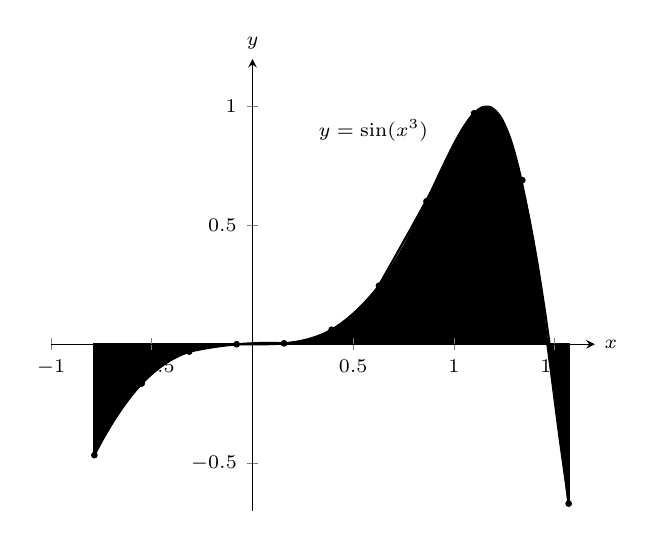
\begin{tikzpicture}
\begin{axis}[width=.7\textwidth,%
tick label style={font=\scriptsize},axis y line=middle,axis x line=middle,name=myplot,axis on top,%
			%x=.37\marginparwidth,
			%y=.37\marginparwidth,
%			xtick=\empty,% 
%			extra x ticks={.5,3},
%			extra x tick labels={$a$,$b$},
%			ytick=\empty,
			%minor y tick num=1,%extra y ticks={-5,-3,...,7},%
%			minor x tick num=4,
			ymin=-.7,ymax=1.2,%
			xmin=-1,xmax=1.7%
]

\addplot [{\coloronefill},fill={\coloronefill}] coordinates {(-0.7854,-0.4657)  (-0.7373,-0.3902) (-0.6892,-0.3216)
(-0.6411,-0.2605)  (-0.5931,-0.2071) (-0.5450,-0.1611)
(-0.4969,-0.1224)  (-0.4488,-0.0903) (-0.4007,-0.0643)
(-0.3526,-0.0438)  (-0.3045,-0.0282) (-0.2565,-0.0169)
(-0.2084,-0.0090)  (-0.1603,-0.0041) (-0.1122,-0.0014)
(-0.0641,-0.0003)  (-0.0160,-0.0000) (0.0321,0.0000)
(0.0801,0.0005)  (0.1282,0.0021) (0.1763,0.0055)
(0.2244,0.0113)  (0.2725,0.0202) (0.3206,0.0329)
(0.3687,0.0501)  (0.4167,0.0723) (0.4648,0.1003)
(0.5129,0.1345)  (0.5610,0.1756) (0.6091,0.2240)
(0.6572,0.2800)  (0.7053,0.3436) (0.7533,0.4146)
(0.8014,0.4923)  (0.8495,0.5754) (0.8976,0.6618)
(0.9457,0.7485)  (0.9938,0.8313) (1.0419,0.9048)
(1.0899,0.9622)  (1.1380,0.9953) (1.1861,0.9952)
(1.2342,0.9526)  (1.2823,0.8589) (1.3304,0.7082)
(1.3785,0.4989)  (1.4265,0.2363) (1.4746,-0.0650)
(1.5227,-0.3793)  (1.5708,-0.6700) }
|-(axis cs:-0.7854,0 )--cycle;

\addplot [{\colorone},thick,smooth] coordinates {(-0.7854,-0.4657)  (-0.7373,-0.3902) (-0.6892,-0.3216)
(-0.6411,-0.2605)  (-0.5931,-0.2071) (-0.5450,-0.1611)
(-0.4969,-0.1224)  (-0.4488,-0.0903) (-0.4007,-0.0643)
(-0.3526,-0.0438)  (-0.3045,-0.0282) (-0.2565,-0.0169)
(-0.2084,-0.0090)  (-0.1603,-0.0041) (-0.1122,-0.0014)
(-0.0641,-0.0003)  (-0.0160,-0.0000) (0.0321,0.0000)
(0.0801,0.0005)  (0.1282,0.0021) (0.1763,0.0055)
(0.2244,0.0113)  (0.2725,0.0202) (0.3206,0.0329)
(0.3687,0.0501)  (0.4167,0.0723) (0.4648,0.1003)
(0.5129,0.1345)  (0.5610,0.1756) (0.6091,0.2240)
(0.6572,0.2800)  (0.7053,0.3436) (0.7533,0.4146)
(0.8014,0.4923)  (0.8495,0.5754) (0.8976,0.6618)
(0.9457,0.7485)  (0.9938,0.8313) (1.0419,0.9048)
(1.0899,0.9622)  (1.1380,0.9953) (1.1861,0.9952)
(1.2342,0.9526)  (1.2823,0.8589) (1.3304,0.7082)
(1.3785,0.4989)  (1.4265,0.2363) (1.4746,-0.0650)
(1.5227,-0.3793)  (1.5708,-0.6700) };

\addplot [{\colortwo},domain=-.785:-.314,thick] {-.11-.721*x-1.49*x^2};
\addplot [thick,{\colortwo}] coordinates {(-.785,-.466) (-.785,0) (-.314,0) (-.314,-.03)};

\addplot [{\colortwo},domain=-.314:.157,thick] {.004+.037*x-.236*x^2};
\addplot [thick,{\colortwo}] coordinates {(-.314,0) (.157,0) (.157,.004)};

\addplot [{\colortwo},domain=.157:.628,thick] {.037-.395*x+1.156*x^2};
\addplot [thick,{\colortwo}] coordinates {(.157,0) (.628,0) (.628,.246)};

\addplot [{\colortwo},domain=.628:1.1,thick] {-.632+1.32*x+.13*x^2};
\addplot [thick,{\colortwo}] coordinates {(.628,0) (1.1,0) (1.1,.971)};

\addplot [{\colortwo},domain=1.1:1.57,thick] {-11.98+22.46*x-9.72*x^2};
\addplot [thick,{\colortwo}] coordinates {(1.1,0) (1.57,0) (1.57,-.67)};

\filldraw (axis cs:-.785,-.466 ) circle (1pt)
					(axis cs:-.55,-.165 ) circle (1pt)
					(axis cs:-.314,-.031 ) circle (1pt)
					(axis cs:-.0785,0 ) circle (1pt)
					(axis cs:.157,.004 ) circle (1pt)
					(axis cs:.393,.061 ) circle (1pt)
					(axis cs:.628,.246 ) circle (1pt)
					(axis cs:.864,.601 ) circle (1pt)
					(axis cs:1.1,.971 ) circle (1pt)
					(axis cs:1.34,.69 ) circle (1pt)
					(axis cs:1.57,-.67 ) circle (1pt);

\draw (axis cs:.6,.9) node {\scriptsize $y=\sin(x^3)$};
\end{axis}

\node [right] at (myplot.right of origin) {\scriptsize $x$};
\node [above] at (myplot.above origin) {\scriptsize $y$};
\end{tikzpicture}
}

Recall that the actual value, accurate to $ 3 $ decimal places, is $ 0.460 $. Our approximation is within one 1/100$^\text{th}$ of the correct value. The graph in Figure \ref{fig:num6b} shows how closely the parabolas match the shape of the graph.
}
\end{solution}





\subsection{Summary and Error Analysis}

We summarize the key concepts of this section thus far in the following Key Idea.

\begin{formulabox}[Numerical Integration] \label{idea:numerical}
{Let $f$ be a continuous function on $[a,b]$, let $n$ be a positive integer, and let $\ds\dx = \frac{b-a}{n}$. \index{integration!numerical!Left/Right Hand Rule}\index{integration!numerical!Trapezoidal Rule}\index{integration!numerical!Simpson's Rule}
\index{Left/Right Hand Rule}\index{Trapezoidal Rule}\index{Simpson's Rule}
\index{numerical integration!Left/Right Hand Rule}\index{numerical integration!Trapezoidal Rule}\index{numerical integration!Simpson's Rule}

Set $x_1=a$, $x_2 = a+\dx$, $\ldots$, $x_i = a+(i-1)\dx$, $x_{n+1}=b$.

Consider $\ds\int_a^b f(x)\ dx$. 

\parbox{75pt}{Left Hand Rule:} $\ds\int_a^b f(x)\ dx \approx \dx\Big[f(x_0) + f(x_1) + \ldots + f(x_{n-1})\big]$.\\

\parbox{75pt}{Right Hand Rule:} $\ds\int_a^b f(x)\ dx \approx \dx\Big[f(x_1) + f(x_2) + \ldots + f(x_{n})\big]$.\\

\parbox{75pt}{Trapezoidal Rule:} $\ds\int_a^b f(x)\ dx \approx \frac{\dx}2\Big[f(x_0) + 2f(x_1) + 2f(x_2) +\ldots + 2f(x_{n-1})+ f(x_{n})\big]$.\\

\parbox{75pt}{Simpson's Rule:} $\ds\int_a^b f(x)\ dx \approx \frac{\dx}3\Big[f(x_0) + 4f(x_1) + 2f(x_2) +\ldots + 4f(x_{n-1})+ f(x_{n})\big]$ {\small ($n$ even)}.
} 
\end{formulabox}


In our examples, we approximated the value of a definite integral using a given method then compared it to the ``right'' answer. This should have raised several questions in the reader's mind, such as:
\begin{enumerate}
\item		How was the ``right'' answer computed?
\item		If the right answer can be found, what is the point of approximating?
\item		If there is value to approximating, how are we supposed to know if the approximation is any good?
\end{enumerate}

These are good questions, and their answers are educational. In the examples, \textit{the} right answer was never computed. Rather, an approximation accurate to a certain number of places after the decimal was given. In Example \ref{ex_num1}, we do not know the \textit{exact} answer, but we know it starts with 0.7468. These more accurate approximations were computed using numerical integration but with more precision (i.e., more subintervals and the help of a computer). 

Since the exact answer cannot be found, approximation still has its place. How are we to tell if the approximation is any good?

``Trial and error'' provides one way. %(No, this does not refer to seeing whether or not the bridge collapses.) 
Using technology, make an approximation with, say, 10, 100, and 200 subintervals. This likely will not take much time at all, and a trend should emerge. If a trend does not emerge, try using yet more subintervals. Keep in mind that trial and error is never foolproof; you might stumble upon a problem in which a trend will not emerge.


A second method is to use Error Analysis. While the details are beyond the scope of this text, there are some formulas that give \textit{bounds} for how good your approximation will be. For instance, the formula might state that the approximation is within 0.1 of the correct answer. If the approximation is 1.58, then one knows that the correct answer is between 1.48 and 1.68. By using lots of subintervals, one can get an approximation as accurate as one likes. Theorem \ref{thm:numerical_error} states what these bounds are.

%\setboxwidth{50pt}%
%\ifthenelse{\isodd{\thepage}}{}{\hskip -65pt}%
%\noindent\begin{minipage}{\specialboxlength}

\begin{theorem}{Error Bounds in the Trapezoidal and Simpson's Rules}{numericalerror}
\begin{enumerate}
\index{integration!numerical!Trapezoidal Rule}\index{integration!numerical!Simpson's Rule}
\index{Trapezoidal Rule!error bounds}\index{Simpson's Rule!error bounds}
\index{numerical integration!Trapezoidal Rule!error bounds}\index{numerical integration!Simpson's Rule!error bounds}
\item	Let $E_T$ be the error in approximating $\ds \int_a^b f(x)\ dx$ using the Trapezoidal Rule. 
If $f$ has a continuous 2$^\text{nd}$ derivative on $[a,b]$ and $M$ is any upper bound of $\big|\fpp(x)\big|$ on $[a,b]$, then
$$\ds E_T \leq \frac{(b-a)^3}{12n^2}M.$$

\item	Let $E_S$ be the error in approximating $\ds \int_a^b f(x)\ dx$ using Simpson's Rule. 

If $f$ has a continuous 4$^\text{th}$ derivative on $[a,b]$ and $M$ is any upper bound of $\big|f\,^{(4)}\big|$ on $[a,b]$, then
$$E_S \leq \frac{(b-a)^5}{180n^4}M.$$
\end{enumerate}
\end{theorem}

%\theorem{thm:numerical_error}{Error Bounds in the Trapezoidal and Simpson's Rules}%
%\end{minipage}
%\restoreboxwidth

There are some key things to note about this theorem.
\begin{enumerate}
	\item		The larger the interval, the larger the error. This should make sense intuitively.
	\item		The error shrinks as more subintervals are used (i.e., as $n$ gets larger).  
	\item		The error in Simpson's Rule has a term relating to the 4$^{\text{th}}$ derivative of $f$. Consider a cubic polynomial: it's $4^{\text{th}}$ derivative is 0. Therefore, the error in approximating the definite integral of a cubic polynomial with Simpson's Rule is 0 -- Simpson's Rule computes the exact answer!
	\end{enumerate}

We revisit Examples \ref{exa:ex_num3} and \ref{exa:ex_num5} and compute the error bounds using Theorem \ref{thm:numericalerror} in the following example.\\


\begin{example}{Computing error bounds}{ex_num7}{
Find the error bounds when approximating $\ds \int_0^1 e^{-x^2}\ dx$ using the Trapezoidal Rule and 5 subintervals, and using Simpson's Rule with 4 subintervals.}
\end{example}

\begin{solution}
{
\noindent \textbf{Trapezoidal Rule with $n=5$:}

\mfigure{1}{Graphing $\fpp(x)$ in Example \ref{ex_num7} to help establish error bounds.}{fig:num7a}{
\begin{tikzpicture}
\begin{axis}[width=\marginparwidth+25pt,%
tick label style={font=\scriptsize},axis y line=middle,axis x line=middle,name=myplot,axis on top,%
			%x=.37\marginparwidth,
			%y=.37\marginparwidth,
%			xtick=\empty,% 
%			extra x ticks={.5,3},
%			extra x tick labels={$a$,$b$},
%			ytick=\empty,
			%minor y tick num=1,%extra y ticks={-5,-3,...,7},%
%			minor x tick num=4,
			ymin=-2.1,ymax=.7,%
			xmin=-.1,xmax=1.1%
]

\addplot [{\colorone},smooth,thick] coordinates {(0,-2.) (0.1,-1.9405) (0.2,-1.7679) (0.3,-1.4988) (0.4,-1.1589)(0.5,-0.7788) (0.6,-0.3907) (0.7,-0.024505) (0.8,0.29528) (0.9,0.55162) (1.,0.73576)};


\draw (axis cs:.8,-1.5) node {\scriptsize $y=e^{-x^2}(4x^2-2)$};
\end{axis}

\node [right] at (myplot.right of origin) {\scriptsize $x$};
\node [above] at (myplot.above origin) {\scriptsize $y$};
\end{tikzpicture}
}

We start by computing the $2^\text{nd}$ derivative of $f(x) = e^{-x^2}$: $$\fpp(x) = e^{-x^2}(4x^2-2).$$ Figure \ref{fig:num7a} shows a graph of $\fpp(x)$ on $[0,1]$. It is clear that the largest value of $\fpp$, in absolute value, is 2. Thus we let $M=2$ and apply the error formula from Theorem \ref{thm:numerical_error}.

$$E_T = \frac{(1-0)^3}{12\cdot 5^2}\cdot 2 = 0.00\overline{6}.$$

Our error estimation formula states that our approximation of 0.7445 found in Example \ref{exa:ex_num3} is within $ 0.0067 $ of the correct answer, hence we know that
$$0.7445-0.0067 = .7378 \leq \int_0^1e^{-x^2}\ dx \leq 0.7512 = 0.7445 + 0.0067.$$ We had earlier computed the exact answer, correct to 4 decimal places, to be 0.7468, affirming the validity of Theorem \ref{thm:numerical_error}.\\

\noindent\textbf{Simpson's Rule with $n=4$:}


We start by computing the $4^\text{th}$ derivative of $f(x) = e^{-x^2}$: $$f\,^{(4)}(x) = e^{-x^2}(16x^4-48x^2+12).$$ Figure \ref{fig:num7b} shows a graph of $f\,^{(4)}(x)$ on $[0,1]$. It is clear that the largest value of $f\,^{(4)}$, in absolute value, is 12. Thus we let $M=12$ and apply the error formula from Theorem \ref{thm:numerical_error}.

$$E_s = \frac{(1-0)^5}{180\cdot 4^4}\cdot 12 = 0.00026.$$

\mfigure{.8}{Graphing $f\,^{(4)}(x)$ in Example \ref{ex_num7} to help establish error bounds.}{fig:num7b}{\begin{tikzpicture}
\begin{axis}[width=.8\textwidth,%
tick label style={font=\scriptsize},axis y line=middle,axis x line=middle,name=myplot,axis on top,%
			%x=.37\marginparwidth,
			%y=.37\marginparwidth,
%			xtick=\empty,% 
%			extra x ticks={.5,3},
%			extra x tick labels={$a$,$b$},
%			ytick=\empty,
			minor y tick num=4,
			%extra y ticks={-5,-3,...,7},%
%			minor x tick num=4,
			ymin=-8,ymax=13.5,%
			xmin=-.1,xmax=1.1%
]

\addplot [{\colorone},smooth,thick] coordinates {(0,12.) (0.066667,11.735) (0.13333,10.955) (0.2,9.7094)(0.26667,8.0726) (0.33333,6.1424) (0.4,4.0303) (0.46667,1.8543)(0.53333,-0.26997) (0.6,-2.237) (0.66667,-3.9579) (0.73333,-5.3651)(0.8,-6.4153) (0.86667,-7.0902) (0.93333,-7.3955) (1.,-7.3576)};


\draw (axis cs:.7,11) node {\scriptsize $y=e^{-x^2}(16x^4-48x^2+12)$};
\end{axis}

\node [right] at (myplot.right of origin) {\scriptsize $x$};
\node [above] at (myplot.above origin) {\scriptsize $y$};
\end{tikzpicture}
}

Our error estimation formula states that our approximation of $0.7468\overline{3}$ found in Example \ref{exa:ex_num5} is within $ 0.00026 $ of the correct answer, hence we know that
$$0.74683-0.00026 = .74657 \leq \int_0^1e^{-x^2}\ dx \leq 0.74709 = 0.74683 + 0.00026.$$ Once again we affirm the validity of Theorem \ref{thm:numerical_error}.
}\\

\end{solution}




At the beginning of this section we mentioned two main situations where numerical integration was desirable. We have considered the case where an antiderivative of the integrand cannot be computed. We now investigate the situation where the integrand is not known. This is, in fact, the most widely used application of Numerical Integration methods. ``Most of the time'' we observe behavior but do not know ``the'' function that describes it. We instead collect data about the behavior and make approximations based off of this data. We demonstrate this in an example.\\


\begin{example}{Approximating distance traveled}{ex_num8}
{
One of the authors drove his daughter home from school while she recorded their speed every $ 30 $ seconds. The data is given in Figure \ref{fig:num8}. Approximate the distance they travelled.
}
\end{example}

\begin{solution}{
Recall that by integrating a speed function we get distance traveled. We have information about $v(t)$; we will use Simpson's Rule to approximate $\ds \int_a^b v(t)\ dt.$ 

The most difficult aspect of this problem is converting the given data into the form we need it to be in. The speed is measured in miles per hour, whereas the time is measured in 30 second increments. 

\mtable{.9}{Speed data collected at 30 second intervals for Example \ref{ex_num8}.}{fig:num8}{%
\begin{tabular}{cc}
Time & \parbox{30pt}{\centering Speed \\ (mph)}\rule[-9pt]{0pt}{5pt} \\ \hline
0 & 0 \\
 1 & 25 \\ 2 & 22 \\
 3 & 19 \\ 4 & 39 \\
 5 & 0 \\ 6 & 43\\
 7 & 59 \\ 8 & 54 \\
 9 & 51 \\ 10 & 43 \\
 11 & 35 \\ 12 & 40 \\
 13 & 43 \\ 14 & 30 \\
 15 & 0 \\ 16 & 0 \\
 17 & 28 \\ 18 & 40 \\
 19 & 42 \\ 20 & 40 \\
 21 & 39 \\ 22 & 40 \\
 23 & 23 \\ 24 & 0 \\ 
\end{tabular}
}
We need to compute $\dx = (b-a)/n$. Clearly, $n=24$. What are $a$ and $b$? Since we start at time $t=0$, we have that $a=0$. The final recorded time came after 24 periods of 30 seconds, which is 12 minutes or 1/5 of an hour. Thus we have
$$\dx = \frac{b-a}{n} = \frac{1/5-0}{24} = \frac1{120}; \quad \frac{\dx}{3} = \frac{1}{360}.$$

Thus the distance traveled is approximately:
\begin{align*}
\int_0^{0.2}v(t)\ dt &\approx \frac{1}{360}\Big[f(x_1)+4f(x_2) + 2f(x_3) + \cdots + 4f(x_n)+f(x_{n+1})\Big]\\
					&= \frac{1}{360}\Big[0+4\cdot25+2\cdot 22 + \cdots + 2\cdot40+4\cdot 23 + 0\Big]\\
					&\approx 6.2167 \ \text{miles.}
\end{align*}
We approximate the author drove 6.2 miles. (Because we are sure the reader wants to know, the author's odometer recorded the distance as about 6.05 miles.)
}\\
\end{solution}





%We started this chapter learning about antiderivatives and indefinite integrals. We then seemed to change focus by looking at areas between the graph of a function and the $x$-axis. We defined these areas as the definite integral of the function, using a notation very similar to the notation of the indefinite integral. The Fundamental Theorem of Calculus tied these two seemingly separate concepts together: we can find areas under a curve, i.e., we can evaluate a definite integral, using antiderivatives. 
%
%We ended the chapter by noting that antiderivatives are sometimes more than difficult to find: they are impossible. Therefore we developed numerical techniques that gave us good approximations of definite integrals.
%
%We used the definite integral to compute areas, and also to compute displacements and distances traveled. There is far more we can do than that. In Chapter \ref{chapter:app_of_int} we'll see more applications of the definite integral. Before that, in Chapter \ref{chapter:anti_tech} we'll learn advanced techniques of integration, analogous to learning rules like the Product, Quotient and Chain Rules of differentiation. 

















%We have now seen some of the most generally useful methods
%for discovering antiderivatives, and there are others. 
%Unfortunately, some functions
%have no simple antiderivatives. In such cases, if the value of a
%definite integral is needed it will have to be approximated. We will
%see two methods that work reasonably well and yet are fairly simple;
%in some cases more sophisticated techniques will be needed.
%
%Of course, we already know one way to approximate an integral: If we
%think of the integral as computing an area, we can add up the areas of
%some rectangles. While this is quite simple, it is usually the case
%that a large number of rectangles is needed to get acceptable
%accuracy. A similar approach is much better. We approximate the area
%under a curve over a small interval as the area of a trapezoid. In
%figure~\ref{fig:trapezoid approximation} we see an area under 
%a curve approximated by rectangles and by trapezoids; it is apparent
%that the trapezoids give a substantially better approximation on each
%subinterval. 
%
%\figure[H]
%%\texonly
%\centerline{\vbox{\beginpicture
%\normalgraphs
%%\ninepoint
%\setcoordinatesystem units <1.25truecm,0.5truecm>
%\setplotarea x from 0 to 4.1, y from 0 to 7.1
%\axis left shiftedto x=0 /
%\axis bottom shiftedto y=0 /
%\setquadratic
%\plot 0.000 4.000 0.200 5.368 0.400 6.304 0.600 6.856 0.800 7.072
%1.000 7.000 1.200 6.688 1.400 6.184 1.600 5.536 1.800 4.792
%2.000 4.000 2.200 3.208 2.400 2.464 2.600 1.816 2.800 1.312
%3.000 1.000 3.200 0.928 3.400 1.144 3.600 1.696 3.800 2.632
%4.000 4.000 /
%\setdashes <2pt>
%\putrule from 0 4 to 1 4
%\putrule from 1 7 to 1 0
%\putrule from 1 7 to 2 7
%\putrule from 2 7 to 2 0
%\putrule from 2 4 to 3 4
%\putrule from 3 4 to 3 0
%\putrule from 3 1 to 4 1
%\putrule from 4 1 to 4 0
%\setsolid
%\setcoordinatesystem units <1.25truecm,0.5truecm> point at -6 0
%\setplotarea x from 0 to 4.1, y from 0 to 7.1
%\axis left shiftedto x=0 /
%\axis bottom shiftedto y=0 /
%\setquadratic
%\plot 0.000 4.000 0.200 5.368 0.400 6.304 0.600 6.856 0.800 7.072
%1.000 7.000 1.200 6.688 1.400 6.184 1.600 5.536 1.800 4.792
%2.000 4.000 2.200 3.208 2.400 2.464 2.600 1.816 2.800 1.312
%3.000 1.000 3.200 0.928 3.400 1.144 3.600 1.696 3.800 2.632
%4.000 4.000 /
%\setlinear
%\setdashes <2pt>
%\plot 0 4 1 7 2 4 3 1 4 4 /
%\putrule from 1 0 to 1 7
%\putrule from 2 0 to 2 4
%\putrule from 3 0 to 3 1
%\putrule from 4 0 to 4 4
%\endpicture}}
%%\htmlfigure{Integration_techniques-numerical_rectangles_trapezoids.html}
%\caption{\label{fig:trapezoid approximation}
%Approximating an area with rectangles and with trapezoids.}
%\endfigure
%
%As with rectangles, we divide the interval into $n$ equal subintervals
%of length $\Delta x$.
%A typical trapezoid is pictured in figure~\ref{fig:one trapezoid};
%it has area $$\ds{f(x_i)+f(x_{i+1})\over2}\Delta x.$$ 
%If we add up the
%  areas of all trapezoids we get
%$${f(x_0)+f(x_1)\over2}\Delta x+{f(x_1)+f(x_2)\over2}\Delta x+\cdots+
%  {f(x_{n-1})+f(x_n)\over2}\Delta x$$
%  $$=\left({f(x_0)\over2}+f(x_1)+f(x_2)+\cdots+f(x_{n-1})+{f(x_n)\over2}\right)
%  \Delta x.$$
%For a modest number of subintervals this is not too difficult to do
%with a calculator; a computer can easily do many subintervals.
%
%\figure[H]
%\centerline{\vbox{\beginpicture
%\normalgraphs
%%\ninepoint
%\setcoordinatesystem units <1.25truecm,0.5truecm>
%\setplotarea x from 0 to 3.0, y from 0 to 7.1
%\axis bottom shiftedto y=0 ticks length <2pt> 
%  withvalues {$x_i$} {$x_{i+1}$} / at 1 2 / /
%\put {$(x_i,f(x_i))$} [r] <-3pt,0pt> at 1 7
%\put {$(x_{i+1},f(x_{i+1}))$} [l] <3pt,0pt> at 2 4
%\setquadratic
%\plot 1.000 7.000 1.167 6.755 1.333 6.370 1.500 5.875 1.667 5.296
%1.833 4.662 2.000 4.000 /
%\setlinear
%\setdashes <2pt>
%\plot 1 7 2 4  /
%\putrule from 2 0 to 2 4
%\putrule from 1 0 to 1 7
%\endpicture}}
%%\endtexonly
%%\figrdef{fig:one trapezoid}
%%\htmlfigure{Integration_techniques-numerical_one_trapezoid.html}
%\caption{\label{fig:one trapezoid}
%A single trapezoid.}
%\endfigure
%
%In practice, an approximation is useful only if we know how accurate
%it is; for example, we might need a particular value accurate to three
%decimal places. When we compute a particular approximation to an
%integral, the error is the difference between the approximation and
%the true value of the integral. For any approximation technique, we
%need an \dfont{error bound}, a value that
%is guaranteed to be larger than the actual error. If $A$ is an
%approximation and $E$ is the associated error bound, then we know
%that the true value of the integral is between $A-E$ and
%$A+E$. In the case of our approximation of the integral, we want
%$E=E(\Delta x)$ to be a function of $\Delta x$ that gets small rapidly
%as $\Delta x$ gets small. Fortunately, for many functions, there is
%such an error bound associated with the trapezoid approximation.
%
%\begin{theorem}{Error for Trapezoid Approximation}{Error for Trapezoid Approximation}\label{Error for Trapezoid Approximation}
%Suppose $f$ has a second derivative $f''$ everywhere on the
%interval $[a,b]$, and $|f''(x)|\le M$ for all $x$ in the
%interval. With $\Delta x= (b-a)/n$, an error bound for the
%trapezoid approximation is
%$$
%  E(\Delta x) = {b-a\over12}M(\Delta x)^2={(b-a)^3\over 12n^2}M.
%$$
%\end{theorem}
%Let's see how we can use this. 
%
%\begin{example}{Approximate an Integral With Trapezoids}{Approximate an Integral With Trapezoids}\label{Approximate an Integral With Trapezoids}
%Approximate $\ds\int_0^1 e^{-x^2}\,dx$ to two decimal places.
%\end{example}
%
%\begin{solution}
%The second derivative of $\ds f=e^{-x^2}$ is $\ds(4x^2-2)e^{-x^2}$, and
%it is not hard to see that on $[0,1]$ $|f''(x)|$ has a maximum value of 2, thus
%we begin by estimating the number of subintervals we are likely to
%need. To get two decimal places of accuracy, we will certainly need
%$E(\Delta x)<0.005$ or
%\begin{eqnarray*}
%  {1\over12}(2){1\over n^2} &<& 0.005\cr
%  {1\over6}(200)&<&n^2\cr
%  5.77\approx\sqrt{100\over3}&<&n
%\end{eqnarray*}
%With $n=6$, the error bound is thus $\ds1/6^3<0.0047$.
%We compute the trapezoid approximation for six intervals:
%$$
%  \left({f(0)\over2}+f(1/6)+f(2/6)+\cdots+f(5/6)+{f(1)\over2}\right){1\over6}
%  \approx 0.74512.
%$$
%So the true value of the integral is between $0.74512-0.0047=0.74042$ and
%$0.74512+0.0047=0.74982$. Unfortunately, the first rounds to $0.74$
%and the second 
%rounds to $0.75$, so we can't be sure of the correct value in
%the second decimal place; we need to pick a larger $n$.
%As it turns out, we need to go to $n=12$ to get two bounds that both
%round to the same value, which turns out to be $0.75$. For comparison,
%using $12$ rectangles to approximate the area gives $0.7727$, which is
%considerably less accurate than the approximation using six trapezoids.
%
%In practice it
%generally pays to start by requiring better than the maximum possible
%error; for example, we might have initially required $E(\Delta
%x)<0.001$, or 
%\begin{eqnarray*}
%  {1\over12}(2){1\over n^2} &<& 0.001\cr
%  {1\over6}(1000)&<&n^2\cr
%  12.91\approx\sqrt{500\over3}&<&n
%\end{eqnarray*}
%Had we immediately tried $n=13$ this would have given us the desired
%answer. 
%\end{solution}
%
%The trapezoid approximation works well, especially compared to
%rectangles, because the tops of the trapezoids form a reasonably good
%approximation to the curve when $\Delta x$ is fairly small. We can
%extend this idea: what if we try to approximate the curve more
%closely by using something other than a straight line? The obvious
%candidate is a parabola: If we can approximate a short piece of the
%curve with a parabola with equation $\ds y=ax^2+bx+c$, we can easily
%compute the area under the parabola.
%
%There are an infinite number of parabolas through any two given
%points, but only one through three given points. If we find a parabola
%through three consecutive points $(x_i,f(x_i))$,
%$(x_{i+1},f(x_{i+1}))$, $(x_{i+2},f(x_{i+2}))$ on the curve, it should
%be quite close to the curve over the whole interval $[x_i,x_{i+2}]$,
%as in Figure~\ref{fig:one parabola}. If we divide the interval
%$[a,b]$ into an even number of subintervals, we can then approximate
%the curve by a sequence of parabolas, each covering two of the
%subintervals. For this to be practical, we would like a simple formula
%for the area under one parabola, namely, the parabola through
%$(x_i,f(x_i))$, $(x_{i+1},f(x_{i+1}))$, and
%$(x_{i+2},f(x_{i+2}))$. That is, we should attempt to write down the
%parabola $y=ax^2+bx+c$ through these points and then integrate it, and
%hope that the result is fairly simple. Although the algebra involved
%is messy, this turns out to be possible. The algebra is well within
%the capability of a good computer algebra system like Sage, so we will
%present the result without all of the algebra.
%
%To find the parabola, we solve these three equations
%for $a$, $b$, and $c$:
%\begin{eqnarray*}
%  f(x_i)&=&a(x_{i+1}-\Delta x)^2+b(x_{i+1}-\Delta x)+c\cr
%  f(x_{i+1})&=&a(x_{i+1})^2+b(x_{i+1})+c\cr
%  f(x_{i+2})&=&a(x_{i+1}+\Delta x)^2+b(x_{i+1}+\Delta x)+c
%\end{eqnarray*}
%
%Not surprisingly, the solutions turn out to be quite
%messy. Nevertheless, Sage can easily compute and simplify the integral
%to get
%$$
%  \int_{x_{i+1}-\Delta x}^{x_{i+1}+\Delta x} ax^2+bx+c\,dx=
%  {\Delta x\over3}(f(x_i)+4f(x_{i+1})+f(x_{i+2})).
%$$
%Now the sum of the areas under all parabolas is
%$$
%  \displaylines{
%  {\Delta x\over3}(f(x_0)+4f(x_{1})+f(x_{2})+f(x_2)+4f(x_{3})+f(x_{4})+\cdots
%  +f(x_{n-2})+4f(x_{n-1})+f(x_{n}))=\cr
%  {\Delta x\over3}(f(x_0)+4f(x_{1})+2f(x_{2})+4f(x_{3})+2f(x_{4})+\cdots
%  +2f(x_{n-2})+4f(x_{n-1})+f(x_{n})).\cr}
%$$
%
%This is just slightly more complicated than the formula for
%trapezoids; we need to remember the alternating 2 and 4 coefficients, and that the interval must be divided into an \emph{even} number of subintervals.
%This approximation technique is referred to as \dfont{Simpson's Rule}.
%
%\figure[H]
%%\texonly
%\centerline{\vbox{\beginpicture
%\normalgraphs
%%\ninepoint
%\setcoordinatesystem units <3truecm,8truecm>
%\setplotarea x from 0.8 to 2.2, y from 0 to 0.4
%\axis bottom shiftedto y=0 ticks length <2pt> 
%  withvalues {$x_i$} {$x_{i+1}$} {$x_{i+2}$} / at 1 1.5 2 / /
%\put {$(x_i,f(x_i))$} [r] <-3pt,0pt> at 1 0.163
%\put {$(x_{i+2},f(x_{i+2}))$} [l] <3pt,0pt> at 2 0.381
%\setquadratic
%\plot 1.000 0.163 1.050 0.138 1.100 0.120 1.150 0.109 1.200 0.102
%1.250 0.100 1.300 0.102 1.350 0.107 1.400 0.116 1.450 0.128
%1.500 0.142 1.550 0.158 1.600 0.177 1.650 0.197 1.700 0.219
%1.750 0.243 1.800 0.268 1.850 0.295 1.900 0.322 1.950 0.351
%2.000 0.381 /
%\setdashes <2pt>
%\plot 
%1.000 0.162 1.050 0.149 1.100 0.137 1.150 0.129 1.200 0.123
%1.250 0.120 1.300 0.119 1.350 0.121 1.400 0.125 1.450 0.132
%1.500 0.142 1.550 0.154 1.600 0.169 1.650 0.186 1.700 0.206
%1.750 0.229 1.800 0.254 1.850 0.282 1.900 0.312 1.950 0.346
%2.000 0.381 /
%\endpicture}}
%%\caption
%%{A parabola (dashed) approximating a curve (solid).
%%(\expandafter\url\expandafter{\liveurl jsxgraph/numerical_int.html}%
%%AP\endurl)}
%%\endcaption
%%\endtexonly
%%\figrdef{fig:one parabola}
%%\htmlfigure{Integration_techniques-numerical_one_parabola.html}
%\caption{\label{fig:one parabola}
%A parabola (dashed) approximating a curve (solid).}
%\endfigure
%
%\noindent As with the trapezoid method, this is useful only with an error
%bound:
%
%\begin{theorem}{Error for Simpson's Approximation}{Error for Simpson's Approximation}\label{Error for Simpson's Approximation}
%Suppose $f$ has a fourth derivative $f^{(4)}$ everywhere on the
%interval $[a,b]$, and $|f^{(4)}(x)|\le M$ for all $x$ in the
%interval. With $\Delta x= (b-a)/n$, an error bound for Simpson's
%approximation is
%$$
%  E(\Delta x) = {b-a\over180}M(\Delta x)^4={(b-a)^5\over 180n^4}M.
%$$
%\end{theorem}
%
%\begin{example}{Approximate an Integral With Parabolas}{Approximate an Integral With Parabolas}\label{Approximate an Integral With Parabolas}
%Let us again approximate $\ds\int_0^1 e^{-x^2}\,dx$ to two
%decimal places.  
%\end{example}
%
%\begin{solution}
%The fourth derivative of $\ds f=e^{-x^2}$ is
%$\ds(16x^4-48x^2+12)e^{-x^2}$; on $[0,1]$ this is at most
%$12$ in absolute value.  We begin by estimating the number of
%subintervals we are likely to need. To get two decimal places of
%accuracy, we will certainly need $E(\Delta x)<0.005$, but taking a cue
%from our earlier example, let's require $E(\Delta x)<0.001$:
%\begin{eqnarray*}
%  {1\over180}(12){1\over n^4} &<& 0.001\cr
%  {200\over3}&<n^4\cr
%  2.86\approx\root[4] \of {200\over3}&<&n
%\end{eqnarray*}
%So we try $n=4$, since we need an even number of subintervals. Then
%the error bound is $\ds12/180/4^4<0.0003$ and the approximation is
%$$
%  (f(0)+4f(1/4)+2f(1/2)+4f(3/4)+f(1)){1\over3\cdot4}
%  \approx 0.746855.
%$$
%So the true value of the integral is between $0.746855-0.0003=0.746555$ and
%$0.746855+0.0003=0.7471555$, both of which round to $0.75$.
%\end{solution}
%
%
%
%%%%%%%%%%%%%%%%%%%%%%%%%%%%%%%%%%%%%%%%%%%%
\Opensolutionfile{solutions}[ex]
\section*{Exercises for \ref{sec:Numerical Integration}}

\begin{enumialphparenastyle}



% % % % % % % % % % %
\begin{ex}
For the region given, estimate the area using Simpson's Rule:
\begin{enumerate}
\item	[(a)] where the measurements are in centimetres, taken in $ 1 $ cm increments, and
\item	[(b)] where the measurements are in hundreds of meters, taken in $ 100 $ m increments.
\end{enumerate}

\begin{enumerate}
\item 
\begin{tikzpicture}[yscale=.6]%[width=\marginparwidth+25pt]
%\begin{axis}[width=\marginparwidth+25pt,%
%tick label style={font=\scriptsize},axis y line=middle,axis x line=middle,name=myplot,axis on top,%
%			%x=.37\marginparwidth,
%			%y=.37\marginparwidth,
%			xtick={1,2,3,4,5,6,7,8,9,10,11,12},% 
%%			extra x ticks={12.57},
%%			extra x tick labels={$4\pi$},
%%			ytick=\empty,
%			%minor y tick num=1,%extra y ticks={-5,-3,...,7},%
%%			minor x tick num=4,
%			ymin=-.1,ymax=8.5,%
%			xmin=-.1,xmax=12.5%
%]

\draw [{\colorone},thick,fill={\coloronefill},smooth] plot coordinates {(0,2.)(0.06639,2.527)(0.2407,2.839)(0.4857,3.009)(0.7641,3.112)(1.039,
3.221)(1.294,3.367)(1.532,3.53)(1.759,3.689)(1.98,3.823)(2.2,3.915)(2.
42,3.967)(2.64,3.992)(2.86,4.)(3.08,4.)(3.305,3.987)(3.543,3.93)(3.
808,3.797)(4.107,3.558)(4.45,3.185)(4.815,2.703)(5.17,2.152)(5.483,1.
577)(5.723,1.018)(5.872,0.5022)(5.938,0.02083)(5.93,-0.4363)(5.861,-0.
88)(5.741,-1.319)(5.58,-1.742)(5.389,-2.128)(5.179,-2.456)(4.96,-2.
705)(4.737,-2.865)(4.502,-2.953)(4.243,-2.991)(3.95,-3.)(3.614,-2.999)
(3.244,-2.984)(2.86,-2.935)(2.484,-2.829)(2.137,-2.646)(1.832,-2.378)(
1.558,-2.06)(1.299,-1.734)(1.039,-1.443)(0.7641,-1.222)(0.4857,-0.
9779)(0.2407,-0.5015)(0.06639,0.4201)(0,2.)};

\draw (1,3.22) -- (1,-1.443) node [shift={(-3pt,0pt)},rotate=90,pos=.5] {\scriptsize 4.7};

\draw (2,3.823) -- (2,-2.5) node [shift={(-3pt,0pt)},rotate=90,pos=.5] {\scriptsize 6.3};

\draw (3,4) -- (3,-2.95) node [shift={(-3pt,0pt)},rotate=90,pos=.5] {\scriptsize 6.9};

\draw (4,3.62) -- (4,-3) node [shift={(-3pt,0pt)},rotate=90,pos=.5] {\scriptsize 6.6};

\draw (5,2.4) -- (5,-2.7) node [shift={(-3pt,0pt)},rotate=90,pos=.5] {\scriptsize 5.1};

%\end{axis}
%
%\node [right] at (myplot.right of origin) {\scriptsize $x$};
%\node [above] at (myplot.above origin) {\scriptsize $y$};
\end{tikzpicture}




\item 
\begin{tikzpicture}[yscale=.6]%[width=\marginparwidth+25pt]
%\begin{axis}[width=\marginparwidth+25pt,%
%tick label style={font=\scriptsize},axis y line=middle,axis x line=middle,name=myplot,axis on top,%
%			%x=.37\marginparwidth,
%			%y=.37\marginparwidth,
%			xtick={1,2,3,4,5,6,7,8,9,10,11,12},% 
%%			extra x ticks={12.57},
%%			extra x tick labels={$4\pi$},
%%			ytick=\empty,
%			%minor y tick num=1,%extra y ticks={-5,-3,...,7},%
%%			minor x tick num=4,
%			ymin=-.1,ymax=8.5,%
%			xmin=-.1,xmax=12.5%
%]

\draw [{\colorone},thick,fill={\coloronefill},smooth] plot coordinates {(0,1.)(0.05533,1.541)(0.2027,1.965)(0.414,2.278)(0.6613,2.483)(0.9167,
2.583)(1.157,2.588)(1.382,2.521)(1.595,2.409)(1.799,2.282)(2.,2.167)(
2.2,2.089)(2.4,2.068)(2.6,2.119)(2.8,2.257)(3.,2.5)(3.201,2.847)(3.
411,3.233)(3.636,3.58)(3.885,3.807)(4.167,3.833)(4.483,3.604)(4.815,3.
159)(5.139,2.561)(5.431,1.876)(5.667,1.167)(5.828,0.488)(5.917,-0.
1427)(5.943,-0.7173)(5.912,-1.228)(5.833,-1.667)(5.715,-2.028)(5.564,-
2.317)(5.389,-2.543)(5.199,-2.712)(5.,-2.833)(4.799,-2.912)(4.589,-2.
943)(4.364,-2.917)(4.115,-2.828)(3.833,-2.667)(3.513,-2.432)(3.153,-2.
149)(2.753,-1.851)(2.313,-1.568)(1.833,-1.333)(1.323,-1.155)(0.828,-0.
944)(0.4053,-0.5893)(0.1107,0.02133)(0,1)};

\draw (1,2.6) -- (1,-1.) node [shift={(-3pt,0pt)},rotate=90,pos=.5] {\scriptsize 3.6};

\draw (2,2.167) -- (2,-1.43) node [shift={(-3pt,0pt)},rotate=90,pos=.5] {\scriptsize 3.6};

\draw (3,2.5) -- (3,-2) node [shift={(-3pt,0pt)},rotate=90,pos=.5] {\scriptsize 4.5};

\draw (4,3.8) -- (4,-2.75) node [shift={(-3pt,0pt)},rotate=90,pos=.5] {\scriptsize 6.6};

\draw (5,2.8) -- (5,-2.83) node [shift={(-3pt,0pt)},rotate=90,pos=.5] {\scriptsize 5.6};

%\end{axis}
%
%\node [right] at (myplot.right of origin) {\scriptsize $x$};
%\node [above] at (myplot.above origin) {\scriptsize $y$};
\end{tikzpicture}
\end{enumerate}

\begin{sol}
\begin{enumerate}
\item {\begin{enumerate}
\item		Area is $30.8667$ cm$^2$.
\item		Area is $308,667$ m$^2$.
\end{enumerate}
}

\item {\begin{enumerate}
\item		Area is 25.0667 cm$^2$
\item		Area is 250,667 yd$^2$
\end{enumerate}
}

\end{enumerate}
\end{sol}
\end{ex}
% % % % % % % % % % % %


% % % % % % % % % % %
\begin{ex}
{For each definite integral: 
\begin{enumerate}
\item	[(a)] Approximate the definite integral with the Trapezoidal Rule and $n=4$.
\item	[(b)] Approximate the definite integral with Simpson's Rule and $n=4$.
\item	[(c)] Find the exact value of the integral.
\end{enumerate}
}
\begin{enumerate}
\item {$\ds \int_{-1}^1 x^2\ dx$}

\item {$\ds \int_{0}^{10} 5x\ dx$}

\item {$\ds \int_{0}^{\pi} \sin x\ dx$}

\item {$\ds \int_{0}^{4} \sqrt x\ dx$}

\item {$\ds \int_{0}^{3} (x^3+2x^2-5x+7)\ dx$}

\item {$\ds \int_{0}^{1} x^4\ dx$}

\item {$\ds \int_{0}^{2\pi} \cos x\ dx$}

\item {$\ds \int_{-3}^{3} \sqrt{9-x^2} \ dx$}

\end{enumerate}

\begin{sol}
\begin{enumerate}
\item {\begin{enumerate}
\item		$3/4$
\item		$2/3$
\item		$2/3$
\end{enumerate}
}
\item {\begin{enumerate}
\item		$250$
\item		$250$
\item		$250$
\end{enumerate}
}
\item {\begin{enumerate}
\item		$\frac14(1+\sqrt2)\pi\approx 1.896$
\item		$\frac1{6}(1+2\sqrt{2})\pi\approx 2.005$
\item		$2$
\end{enumerate}
}
\item {\begin{enumerate}
\item		$2+\sqrt2+\sqrt3\approx 5.15$
\item		$2/3(3+\sqrt2+2\sqrt3)\approx 5.25$
\item		$16/3\approx 5.33$
\end{enumerate}
}
\item {\begin{enumerate}
\item		$38.5781$
\item		$147/4\approx 36.75$
\item		$147/4\approx 36.75$
\end{enumerate}
}
\item {\begin{enumerate}
\item		$0.2207$
\item		$0.2005$
\item		$1/5$
\end{enumerate}
}
\item {\begin{enumerate}
\item		$0$
\item		$0$
\item		$0$
\end{enumerate}
}
\item {\begin{enumerate}
\item		$9/2(1+\sqrt3)\approx 12.294$
\item		$3+6\sqrt3\approx 13.392$
\item		$9\pi/2\approx 14.137$
\end{enumerate}
}
\end{enumerate}
\end{sol}

\end{ex}
% % % % % % % % % % % %


% % % % % % % % % % %
\begin{ex}
Approximate the definite integral with the Trapezoidal Rule and Simpson's Rule, with $n=6$.
\begin{enumerate}
\item {$\ds \int_{0}^{1} \cos \big(x^2\big) \ dx$}

\item {$\ds \int_{-1}^{1} e^{x^2} \ dx$}

\item {$\ds \int_{0}^{5} \sqrt{x^2+1} \ dx$}

\item {$\ds \int_{0}^{\pi} x\sin x \ dx$}

\item {$\ds \int_{0}^{\pi/2} \sqrt{\cos x} \ dx$}

\item {$\ds \int_{1}^{4} \ln x \ dx$}

\item {$\ds \int_{-1}^{1} \frac{1}{\sin x+2} \ dx$}

\item {$\ds \int_{0}^{6} \frac{1}{\sin x+2} \ dx$}

\end{enumerate}

\begin{sol}
\begin{enumerate}
\item {Trapezoidal Rule: 	$0.9006$

Simpson's Rule: $0.90452$
}
\item {Trapezoidal Rule: 	$3.0241$

Simpson's Rule: $2.9315$
}
\item {Trapezoidal Rule: 	$13.9604$

Simpson's Rule: $13.9066$
}
\item {Trapezoidal Rule: 	$3.0695$

Simpson's Rule: $3.14295$
}
\item 
{Trapezoidal Rule: 	$1.1703$

Simpson's Rule: $1.1873$
}
\item {Trapezoidal Rule: 	$2.52971$

Simpson's Rule: $2.5447$
}
\item {Trapezoidal Rule: 	$1.0803$

Simpson's Rule: $1.077$
}
\item {Trapezoidal Rule: 	$3.5472$

Simpson's Rule: $3.6133$
}
\end{enumerate}
\end{sol}

\end{ex}
% % % % % % % % % % % %
% % % % % % % % % % %
\begin{ex}
Find $n$ such that the error in approximating the given definite integral is less than $0.0001$ when using:
\begin{enumerate}
\item [(a)] the Trapezoidal Rule
\item [(b)] Simpson's Rule
\end{enumerate}
\begin{enumerate}
\item {$\ds \int_{0}^{\pi} \sin x \ dx$}

\item {$\ds \int_{1}^{4} \frac{1}{\sqrt x} \ dx$}

\item {$\ds \int_{0}^{\pi} \cos \big(x^2\big) \ dx$}

\item {$\ds \int_{0}^{5} x^4 \ dx$}

\end{enumerate}

\begin{sol}
\begin{enumerate}
\item {\begin{enumerate}
\item		$n=161$ (using $\max\big(\fpp(x)\big)=1$)
\item		$n=12$	(using $\max\big(f\,^{(4)}(x)\big)=1$)
\end{enumerate}
}
\item {\begin{enumerate}
\item		$n=150$ (using $\max\big(\fpp(x)\big)=1$)
\item		$n=18$	(using $\max\big(f\,^{(4)}(x)\big)=7$)
\end{enumerate}
}
\item {\begin{enumerate}
\item		$n=1004$ (using $\max\big(\fpp(x)\big)=39$)
\item		$n=62$	(using $\max\big(f\,^{(4)}(x)\big)=800$)
\end{enumerate}
}
\item {\begin{enumerate}
\item		$n=5591$ (using $\max\big(\fpp(x)\big)=300$)
\item		$n=46$	(using $\max\big(f\,^{(4)}(x)\big)=24$)
\end{enumerate}
}
\end{enumerate}
\end{sol}

\end{ex}
% % % % % % % % % % % %

In the following problems, compute the trapezoid and Simpson
approximations using $ 4 $ subintervals, and compute the error bound
for each. (Finding the maximum values of the second and fourth
derivatives can be challenging for some of these; you may use a
graphing calculator or computer software to estimate the maximum
values.) 

%If you have access to Sage or similar software, approximate
%each integral to two decimal places.  You can use this
%\texonly
%\expandafter\url\expandafter{\sageurl simpson_and_trapezoid}% 
%\endurl\ to get started.
%\endtexonly
%\htmlknowl{Integration_techniques-Simpson_and_trapezoid_in_sage.html}{Sage worksheet to get started.}








%%%%%%%%%%
\begin{ex}
 $\ds\int_1^3 x\,dx$
\begin{sol}
 T,S: $4\pm0$
\end{sol}
\end{ex}
%%%%%%%%%%

%%%%%%%%%%
\begin{ex}
 $\ds\int_0^3 x^2\,dx$
\begin{sol}
 T: $9.28125\pm0.281125 $; S: $9\pm0$
\end{sol}
\end{ex}
%%%%%%%%%%

%%%%%%%%%%
\begin{ex}
 $\ds\int_2^4 x^3\,dx$
\begin{sol}
 T: $60.75\pm1$; S: $60\pm0$
\end{sol}
\end{ex}
%%%%%%%%%%

%%%%%%%%%%
\begin{ex}
 $\ds\int_1^3 {1\over x}\,dx$
\begin{sol}
 T: $1.1167\pm 0.0833$; S: $1.1000\pm 0.0167$
\end{sol}
\end{ex}
%%%%%%%%%%

%%%%%%%%%%
\begin{ex}
 $\ds\int_1^2 {1\over 1+x^2}\,dx$
\begin{sol}
 T: $0.3235\pm 0.0026$; S: $0.3217\pm 0.000065$
\end{sol}
\end{ex}
%%%%%%%%%%

%%%%%%%%%%
\begin{ex}
 $\ds\int_0^1 x\sqrt{1+x}\,dx$
\begin{sol}
 T: $0.6478\pm 0.0052$; S: $0.6438\pm 0.000033$
\end{sol}
\end{ex}
%%%%%%%%%%

%%%%%%%%%%
\begin{ex}
 $\ds\int_1^5 {x\over 1+x}\,dx$
\begin{sol}
 T: $2.8833\pm 0.0834$; S: $2.9000\pm 0.0167$
\end{sol}
\end{ex}
%%%%%%%%%%

%%%%%%%%%%
\begin{ex}
 $\ds\int_0^1 \sqrt{x^3+1}\,dx$
\begin{sol}
 T: $1.1170\pm 0.0077$; S: $1.1114\pm 0.0002$
\end{sol}
\end{ex}
%%%%%%%%%%

%%%%%%%%%%
\begin{ex}
 $\ds\int_0^1 \sqrt{x^4+1}\,dx$
\begin{sol}
 T: $1.097\pm 0.0147$; S: $1.089\pm 0.0003$
\end{sol}
\end{ex}
%%%%%%%%%%

%%%%%%%%%%
\begin{ex}
 $\ds\int_1^4 \sqrt{1+1/x}\,dx$
\begin{sol}
 T: $3.63\pm 0.087$; S: $3.62\pm 0.032$
\end{sol}
\end{ex}
%%%%%%%%%%

%%%%%%%%%%
\begin{ex}
 Using Simpson's rule on a parabola $f(x)$, even with just
two subintervals, gives the exact value of the integral, because the
parabolas used to approximate $f$ will be $f$ itself. Remarkably,
Simpson's rule also computes the integral of a cubic function
$f(x)=ax^3+bx^2+cx+d$ exactly. Show this is true by showing that
$$
  \int_{x_0}^{x_2}
  f(x)\,dx={x_2-x_0\over3\cdot2}(f(x_0)+4f((x_0+x_2)/2)+f(x_2)).
$$
This does require a bit of messy algebra, so you may prefer to use Sage.
\end{ex}
%%%%%%%%%%

\end{enumialphparenastyle}